\begin{document}
\chapter{CURVES}

This Supplementary Material provides additional derivations, implementation details and results. More specifically: 
\begin{itemize}[noitemsep]
\item Section A provides supplementary implementation details in the form of:
    \begin{itemize}[noitemsep]
    \item Images of testing set of visual referents;
    \item Topographic score derivation;
    \item Training procedures and hyperparameters;
    \item Pseudo-code.
\end{itemize}

\item Section B provides supplementary results:
    \begin{itemize}[noitemsep]
    \item Auto-comprehension generalization performances;
    \item Additional Lexicons;
    \item Utterances examples across perspectives illustrating coherence;
    \item Topographic maps \& scores;
    \item Composition matrix examples;
    \item T-SNEs of embeddings;
\end{itemize}
\end{itemize}

\section{Supplementary Methods}

\subsection{Testing Set}


\begin{figure}[h!]
\centering 
 \begin{tabular}{ccccc}
     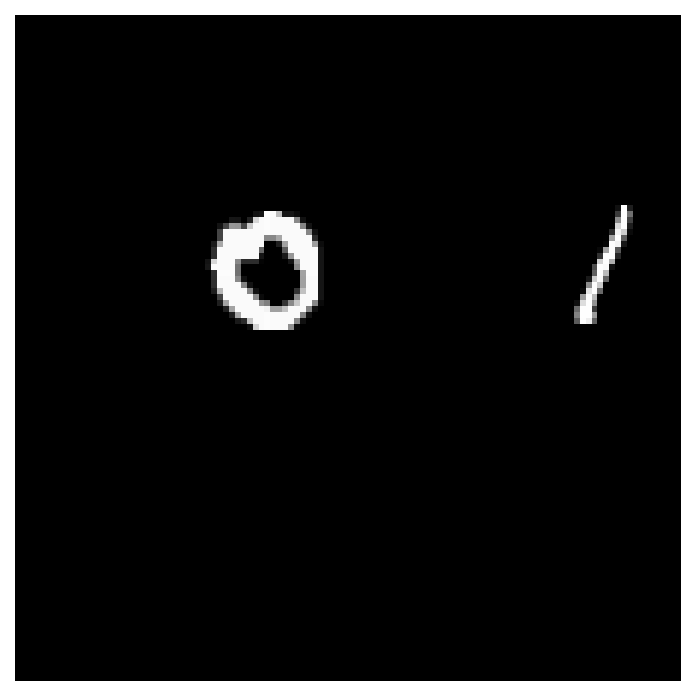
\includegraphics[width=0.12\textwidth]{"curves/R2_examples/0.pdf"} &
     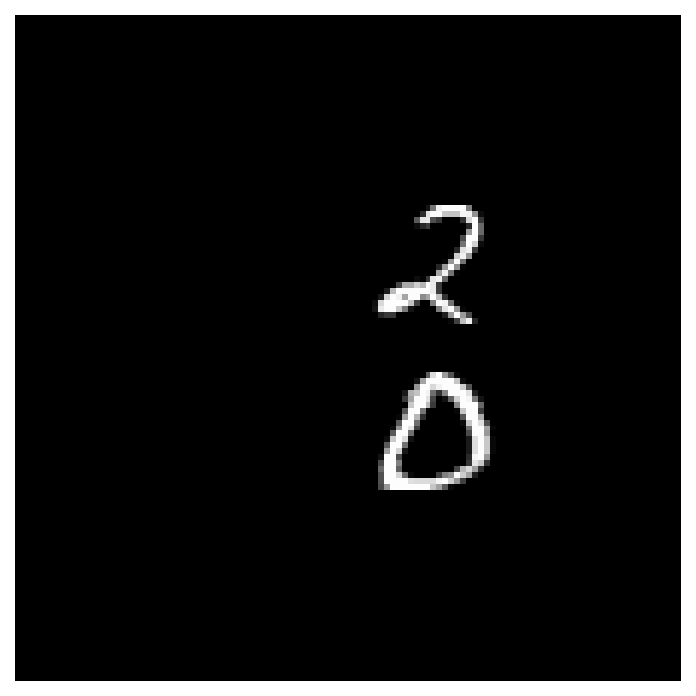
\includegraphics[width=0.12\textwidth]{"curves/R2_examples/1.pdf"} &
     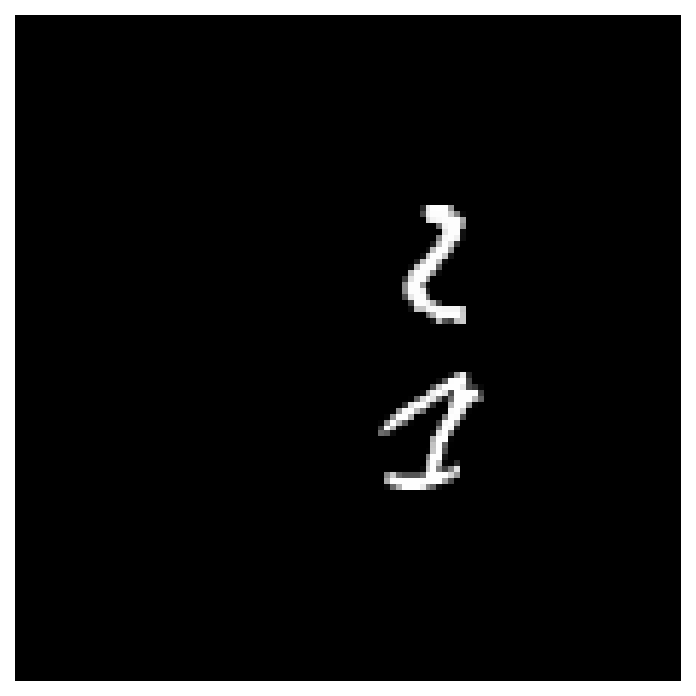
\includegraphics[width=0.12\textwidth]{"curves/R2_examples/2.pdf"} &
     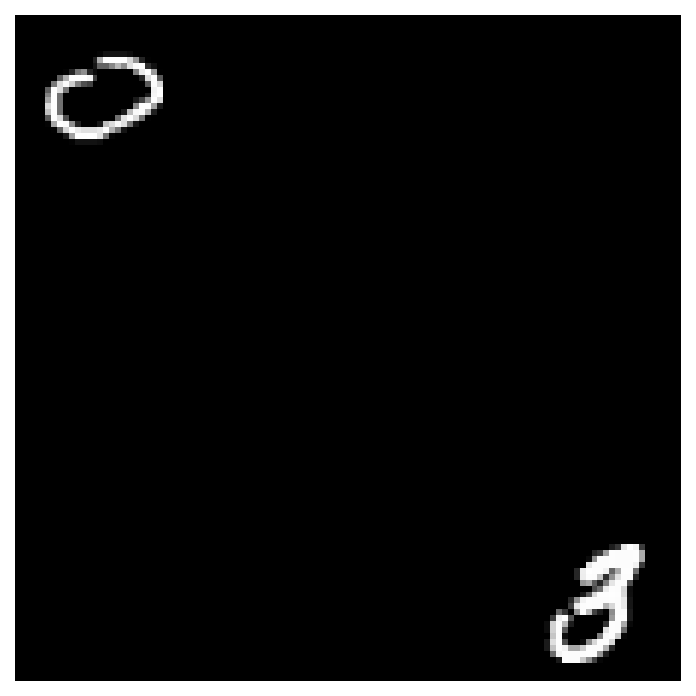
\includegraphics[width=0.12\textwidth]{"curves/R2_examples/3.pdf"} &
     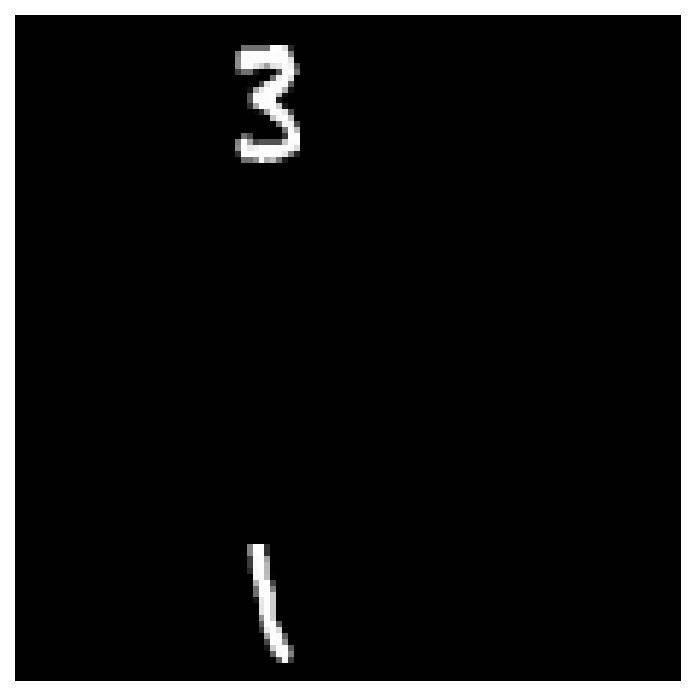
\includegraphics[width=0.12\textwidth]{"curves/R2_examples/4.pdf"} \\
     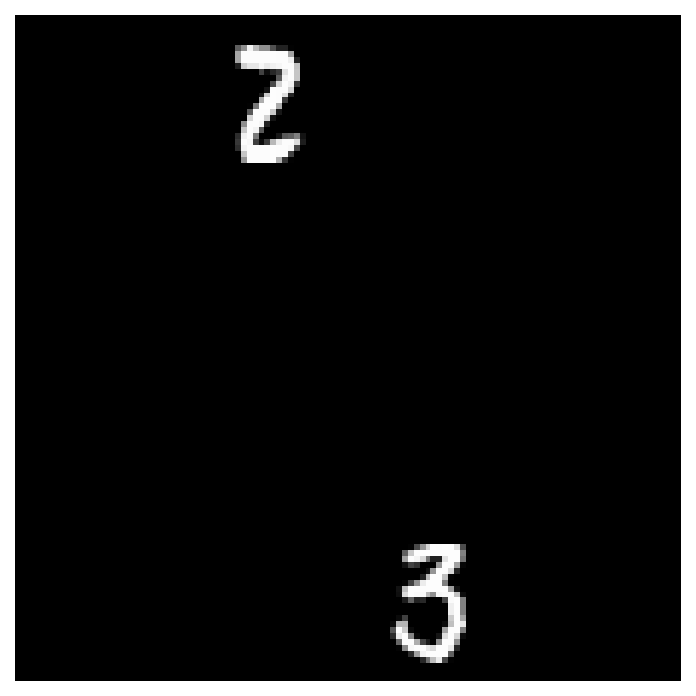
\includegraphics[width=0.12\textwidth]{"curves/R2_examples/5.pdf"} &
     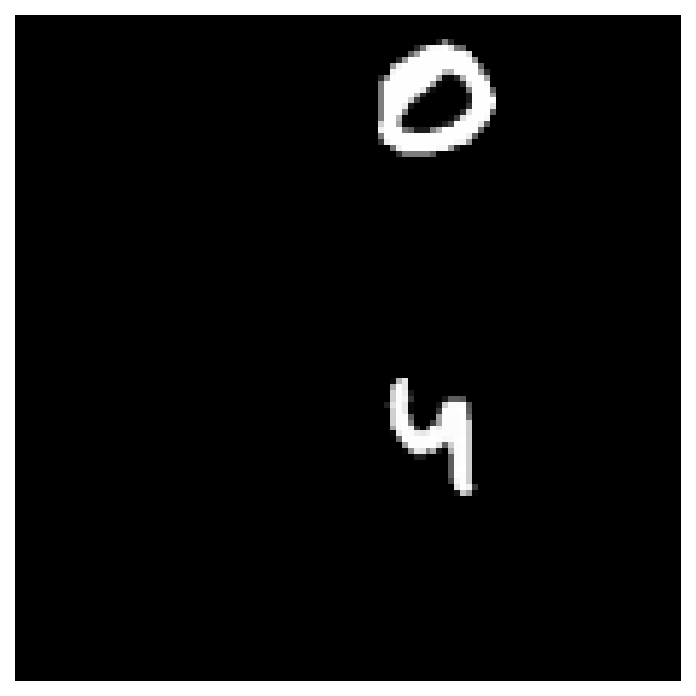
\includegraphics[width=0.12\textwidth]{"curves/R2_examples/6.pdf"} &
     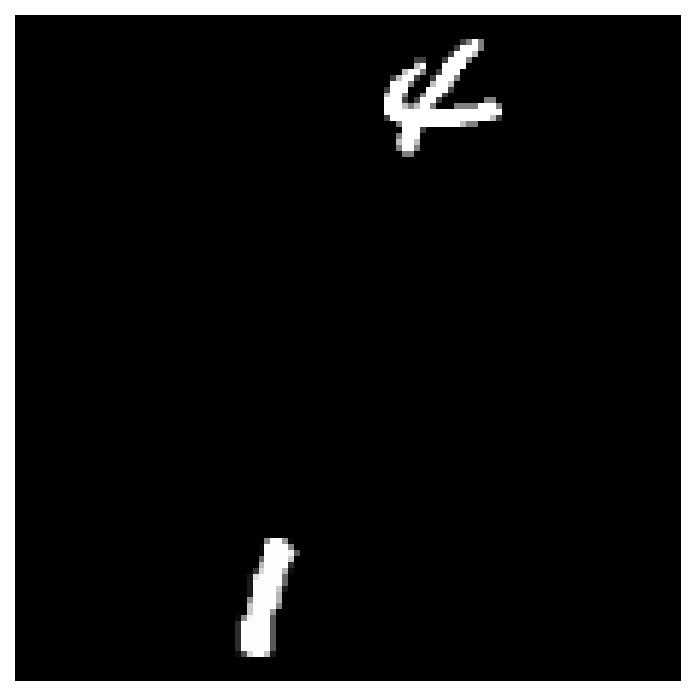
\includegraphics[width=0.12\textwidth]{"curves/R2_examples/7.pdf"} &
     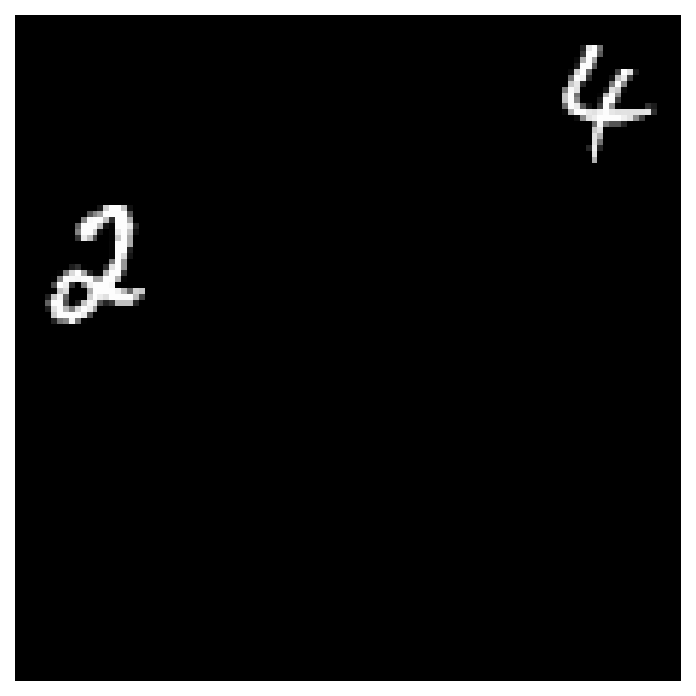
\includegraphics[width=0.12\textwidth]{"curves/R2_examples/8.pdf"} &
     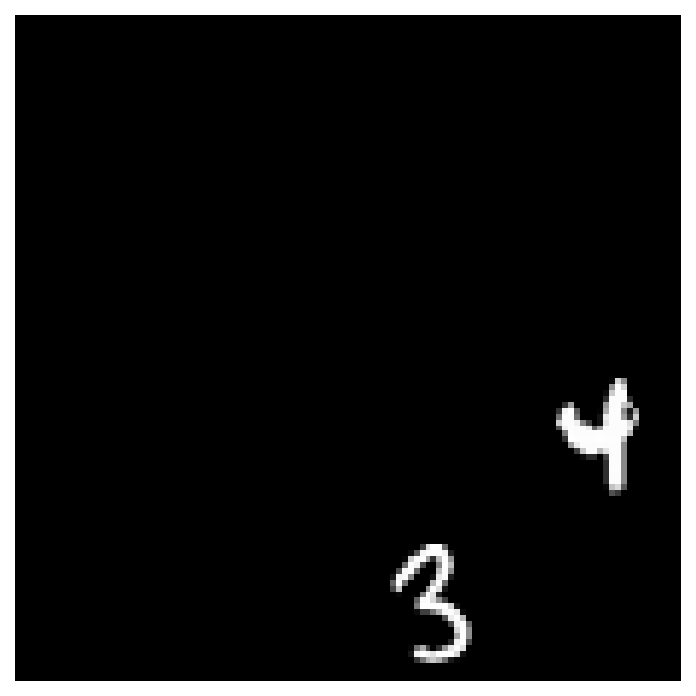
\includegraphics[width=0.12\textwidth]{"curves/R2_examples/9.pdf"}
 \end{tabular}

\caption{\textbf{Perspective instances of the testing set} $\mathcal{R}_5^2$.}
\end{figure}


\label{sup:ref_comp}
\subsection{Topographic Score}
\label{sup:topo_comp}
To evaluate the compositionality of the emerging language we define the topographic score:
\begin{equation}
    \rho_{ij} = ||(O, h_{ij})||_2 - ||(O, h_k)||_2 \text{ with } k = \text{argmin}_{k\in \{i, j\}}||h_k,h_{ij}||_2)
    \label{eq:topo_score}
\end{equation}

It is obtained by computing the Hausdorff distance between the utterances denoting compositional referents with respect to both the utterance denoting the single feature $i$ ($d_H(u(r_i),\cdot)$)and the one denoting the single feature $j$ ($d_H(u(r_j),\cdot)$). To derive our metric, we define 4 groups of utterances denoting compositional referents. 
\begin{itemize}[noitemsep,topsep=0pt]
    \item $u(r_{ij})$ the utterances for referent made of feature $i$ and $j$.
    \item $u(r_{xj}, x\neq i)$ the utterances denoting referent made by composing feature $j$ with any other feature different than $i$
    \item $u(r_{iy}, y\neq j)$ the utterances denoting referent made by composing feature $i$ with any other feature different than $j$
    \item $u(r_{xy})$ the utterance denoting all other compositional referents in $\mathcal{R}^2_5$.
\end{itemize}
%
and compute their Hausdorff distances to $u(r_i)$ and $u(r_j)$.
As displayed in Figure~\ref{fig:topo_distances_intuitive}, if utterances $u(r_{ij})$ are compositional we expect them to be at the same time close to $u(r_{i})$ and close to $u(r_{j})$ and hence to land in the bottom left corner of the distance graph. Moreover, they should be closer to the origin than $u(r_{xj})$ and $u(r_{iy})$. To quantify to what extent it is the case we compute the barycenter of each group $h_i, h_j, h_{ij}$ and $h_{xy}$ and compute "how closer to the origin" is the compositional barycenter $h_{ij}$ compared to its closest barycenter using equation~\ref{eq:topo_score}.
\begin{figure}[h!]
    \centering
    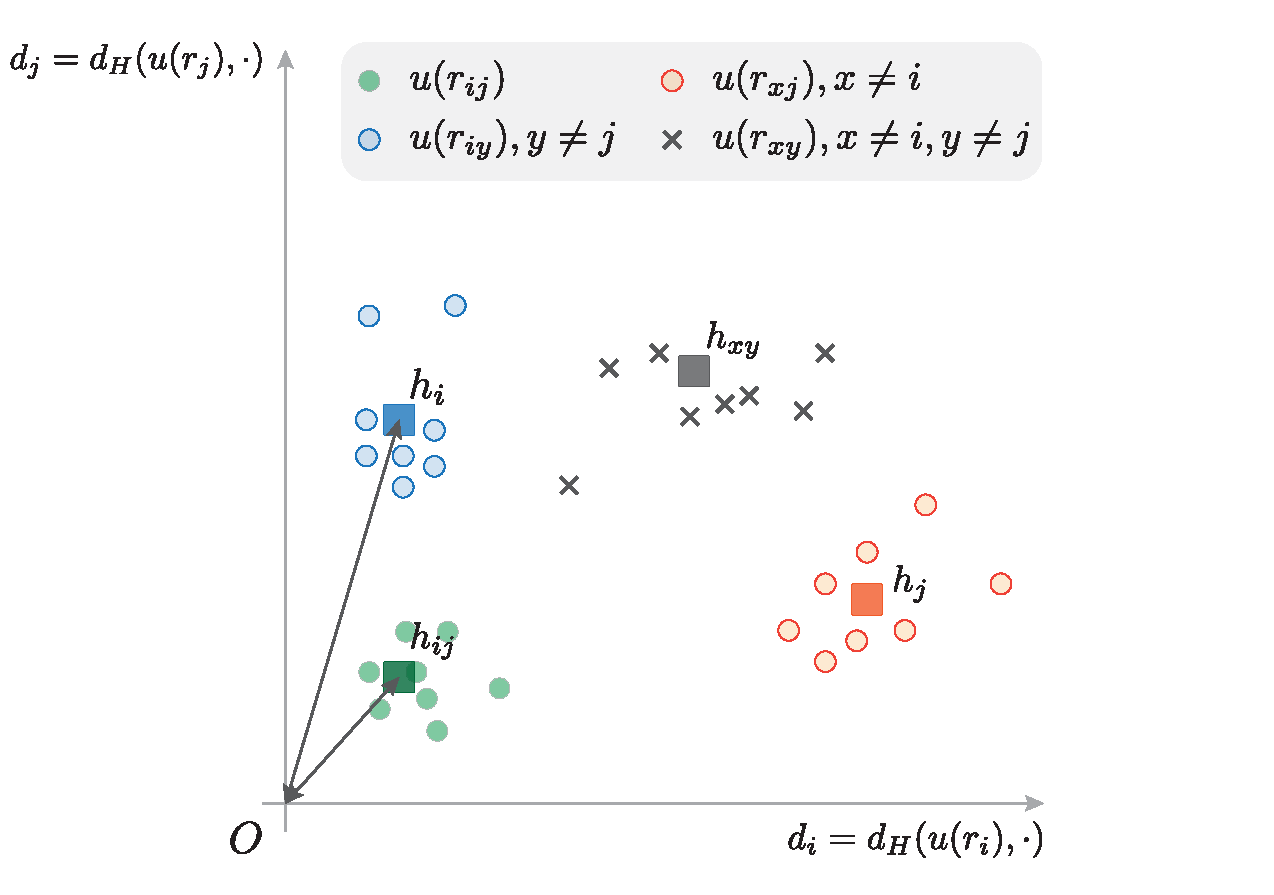
\includegraphics[width=0.7\textwidth]{curves/topographic_map.pdf}
    \caption{Idealized mapping of utterances denoting compositional referents in the plan representing distances to utterances naming isolated features $i$ and $j$.}
    \label{fig:topo_distances_intuitive}
\end{figure}


\subsection{Training procedure and hyperparameters}
\label{sup:training_proc}
Agents have two separate encoders based on the same model architecture described in Table.\ref{table:hyperparameters}. Each agent performs association updates with a single step of gradient descent, using its own Adam optimizer with a learning rate of $1e^{-4}$. To allow faster convergence, agents perform an association update between an abstract referent $r^\star_A$ and an utterance $u$ by using a batch of 64 perspectives $\{\Phi(r^\star_A)\}_{i \in [1,64]}$. From a cognitive science perspective, this is comparable to an agent "walking around" an object to better understand how different perceptions relate to the same object. From a computer science perspective, this is similar to the self-supervised framework of SimCLR~\citep{Chen2020ASF}, where agents learn representation by contrastively aligning the embeddings of an input with these of the same transformed input.

\begin{table}[h!]
\centering 

\def\arraystretch{1.5}
\begin{tabular}{ |c|c|} 
 \hline
 Layer & Activation\\
 \hline
 Conv2D(filters=8, stride=2, padding=1) & ReLU\\ 
 \hline
 Conv2D(filters=16, stride=2, padding=1) & ReLU\\ 
 \hline
 Conv2D(filters=32, stride=2, padding=0) & ReLU\\ 
 \hline
 Linear(128) & ReLU\\
 \hline
 Linear(32) & None\\
 \hline
\end{tabular}

\caption{\textbf{Model architecture used for both the referent and utterance Encoders.} (when referents are one-hot vectors, the 3 Conv2D layers are replaced by a Linear layer with ReLu activation)}

\label{table:hyperparameters}
\end{table}

While the drawing pipeline is fully differentiable, it is highly sensitive to local minima. Thus, we solve equation~\ref{eq:descri_gen} in the descriptive case or equation~\ref{eq:discri_gen} in the discriminative scenario by simultaneously performing gradient descent on a batch of $64$ randomly initialized command vectors over 100 iterations, using a newly initialized Adam optimizer each time with a learning rate of $1e^{-2}$.

\newpage
\subsection{Pseudo-code}



\begin{algorithm}
\caption{Speaker's Utterances}\label{alg:sp}
\begin{algorithmic}

\REQUIRE perceived referents $\tilde{R}_S$, speaker's referent encoder $f_S$, speaker's utterance encoder $g_S$, sensory-motor system $M$

\STATE $Z_r \gets f_S(\tilde{R}_S) $
\STATE $c \sim \textrm{Uniform}()$
\FOR{$i \textrm{ in range} (N_{\textrm{production}})$}
    \STATE $U_S \gets M(c)$
    \STATE $Z_u \gets g_S(U)$
    \STATE $S \gets \textrm{sim}_{\textrm{cos}}(Z_r,Z_u)$
    \STATE $\mathcal{L} \gets \textrm{mean(diag(S))} * (-1)$
    \STATE GD step on $c$ to minimize $\mathcal{L}$
\ENDFOR
\STATE \textrm{\textbf{Return} }$M(c)$
\end{algorithmic}
\end{algorithm}

\begin{algorithm}
\caption{Listener's Selections \& Binary Outcomes}\label{alg:ls}
\begin{algorithmic}

\REQUIRE perceived referents $\tilde{R}_L$, produced utterances $U_S$, listener's referent encoder $f_L$, listener's utterance encoder $g_L$

\STATE $Z_r \gets f_L(\tilde{R}_L) $
\STATE $Z_u \gets g_L(U_S) $
\STATE $S\gets \textrm{sim}_{\textrm{cos}}(Z_r,Z_u)$
\STATE $t \gets \textrm{argmax}(S, \textrm{axis=}1)$
\STATE $o \gets \textbf{0}$
\FOR{$i \textrm{ in range} (N_{\textrm{referents}})$}
    \STATE $o_i \gets \mathds{1}_{[t_i = i]}$
\ENDFOR
\STATE \textrm{\textbf{Return} }$o$
\end{algorithmic}
\end{algorithm}

\begin{algorithm}
\caption{Agents's Association Losses}\label{alg:al}
\begin{algorithmic}

\REQUIRE perceived referents $\tilde{R}_A$, produced utterances $U_A$, outcomes $o$, agent's referent encoder $f_A$, agent's utterance encoder $g_A$

\STATE $Z_r \gets f_A(\tilde{R}_A) $
\STATE $Z_u \gets g_A(U_A) $
\STATE $S\gets \textrm{sim}_{\textrm{cos}}(Z_r,Z_u)$
\STATE $\mathcal{L}_0 \gets CE(S, \textrm{reduction=False})$
\STATE $\mathcal{L}_1 \gets CE(S^{\top},\textrm{reduction=False})$
\STATE $\mathcal{L} \gets (\mathcal{L}_0 + \mathcal{L}_1)/2$
\IF{$A = \textrm{"S"}$} 
    \STATE $\mathcal{L} \gets (\mathcal{L} \cdot o) / N_{\textrm{referents}}$
\\ENDIFELSE 
    \STATE $\mathcal{L} \gets (\mathcal{L} \cdot \textbf{1}) / N_{\textrm{referents}}$
\ENDIF 

\STATE $\textrm{\textbf{Return} } \mathcal{L}$
\end{algorithmic}
\end{algorithm}
\newpage
\section{Supplementary Results}

\subsection{Auto-comprehension generalization performances}
\label{sup:auto_social_perf}

\def\arraystretch{1.5}
\begin{table}[!h]
\centering
    \begin{tabular}{|c|c|c|}
     \hline
     \textbf{Ref.} & \textbf{Auto} & \textbf{Social}\\
     \hline
     One-hot & $0.997 \pm 0.005$ & $0.991 \pm 0.015$ \\
     Visual-shared & $0.862 \pm 0.034$ & $0.559 \pm 0.027$  \\
     Visual-unshared & $0.425 \pm 0.016$ & $0.388 \pm 0.02$  \\
     \hline
    \end{tabular}
    \caption{Descriptive Success Rate}
    \label{tab:disc_auto_social}
\end{table}

\def\arraystretch{1.5}
\begin{table}[!h]
\centering
    \begin{tabular}{|c|c|c|}
     \hline
     \textbf{Ref.} & \textbf{Auto} & \textbf{Social}\\
     \hline
     One-hot & $0.997 \pm 0.005$ & $0.992 \pm 0.009$ \\
     Visual-shared & $0.812 \pm 0.019$ & $0.567 \pm 0.034$  \\
     Visual-unshared & $0.466 \pm 0.019$ & $0.404 \pm 0.019$  \\
     \hline
     
    \end{tabular}
    \caption{Descriminative Success Rate}
    \label{tab:desc_auto_social}
\end{table}

We define the \textbf{Auto} performance metric as the communicative success rate, on test set, for language games involving a single agent playing as both the speaker and listener. We compare \textbf{Auto} and \textbf{Social} performances (the latter involving pairs of different agents, as done until now) in Tables~\ref{tab:desc_auto_social}~\&~\ref{tab:disc_auto_social}.


\subsection{Additional Lexicons}
\label{sup:lexicon_one_hot_shared}


\begin{figure}[h!]

\centering
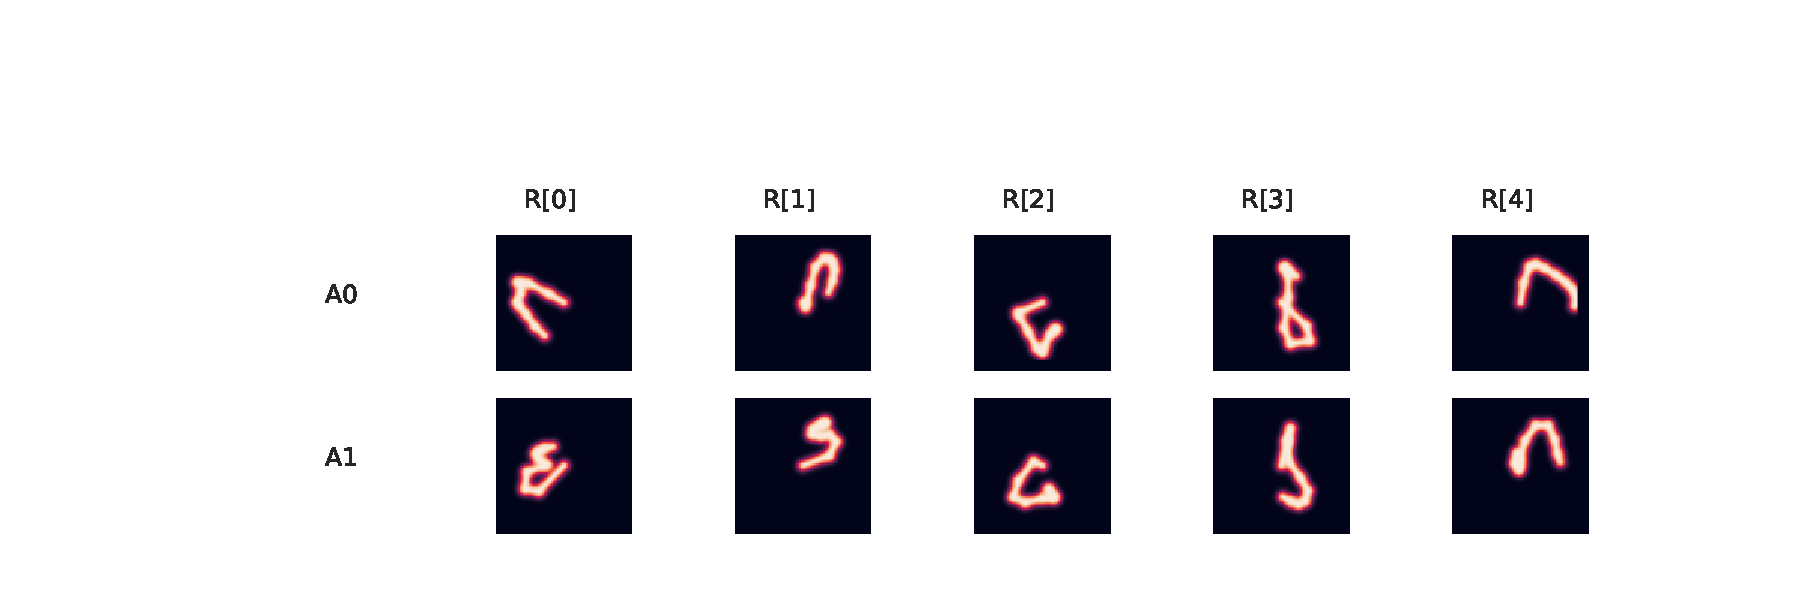
\includegraphics[trim={5cm 1cm 1cm 2cm},clip,width=0.95\textwidth]{curves/training/other_lexicon/Lexicon_SHARED.pdf}
\caption{\textbf{Instance of an emerging lexicon.} (Visual-shared).}
\end{figure}


\begin{figure}[h!]

\centering
    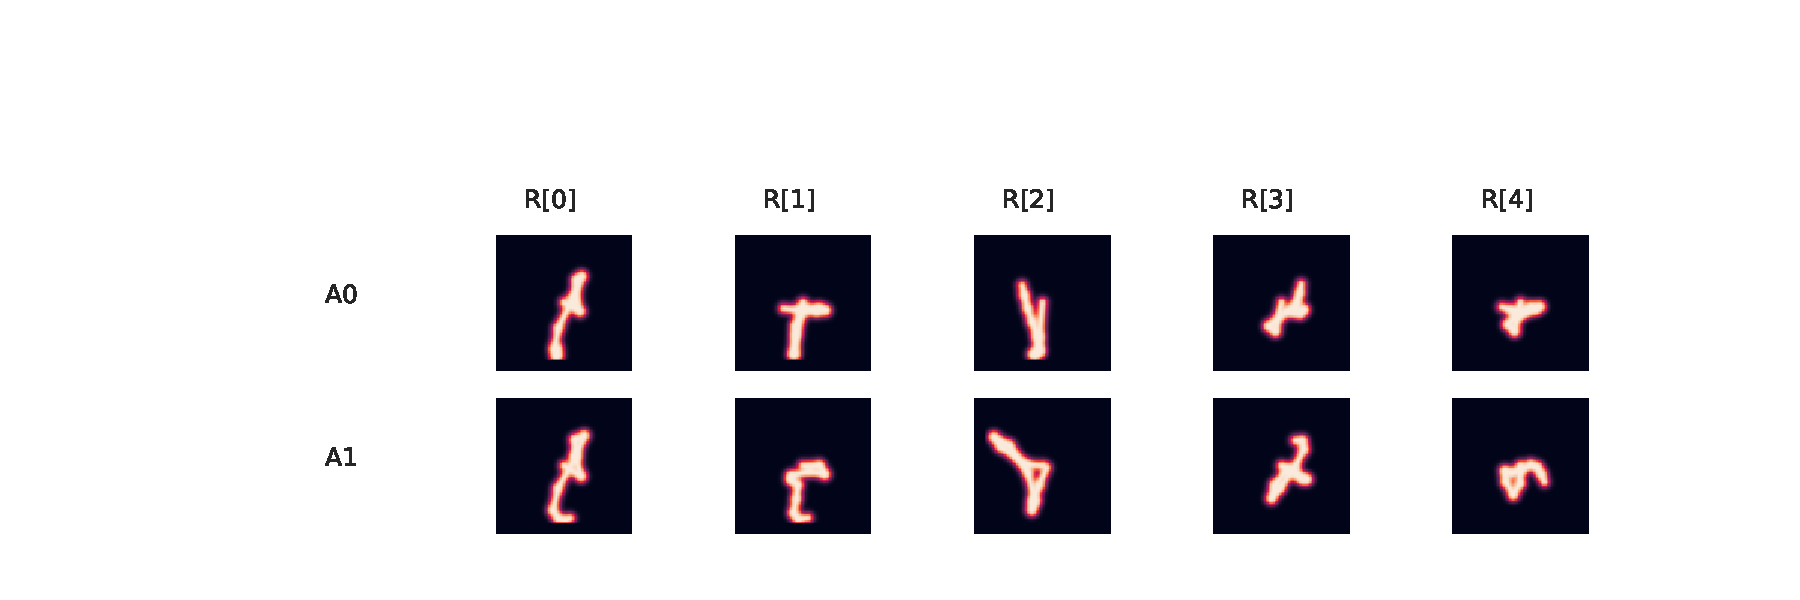
\includegraphics[trim={5cm 1cm 1cm 2cm},clip,width=0.95\textwidth]{curves/training/other_lexicon/Lexicon_ONEHOT.pdf}
    
\caption{\textbf{Instance of an emerging lexicon.} (One-hot).}
\end{figure}

\newpage
\subsection{Utterances examples across perspectives illustrating coherence.}
\label{sup:P-coherence}

The following figures illustrate the P-coherence and A-coherence of an emerging lexicon (Visual-unshared) by displaying, for each referent in $R_1$, the descriptive utterance produced for 10 random perspectives.

\begin{figure}[h!]
\centering
    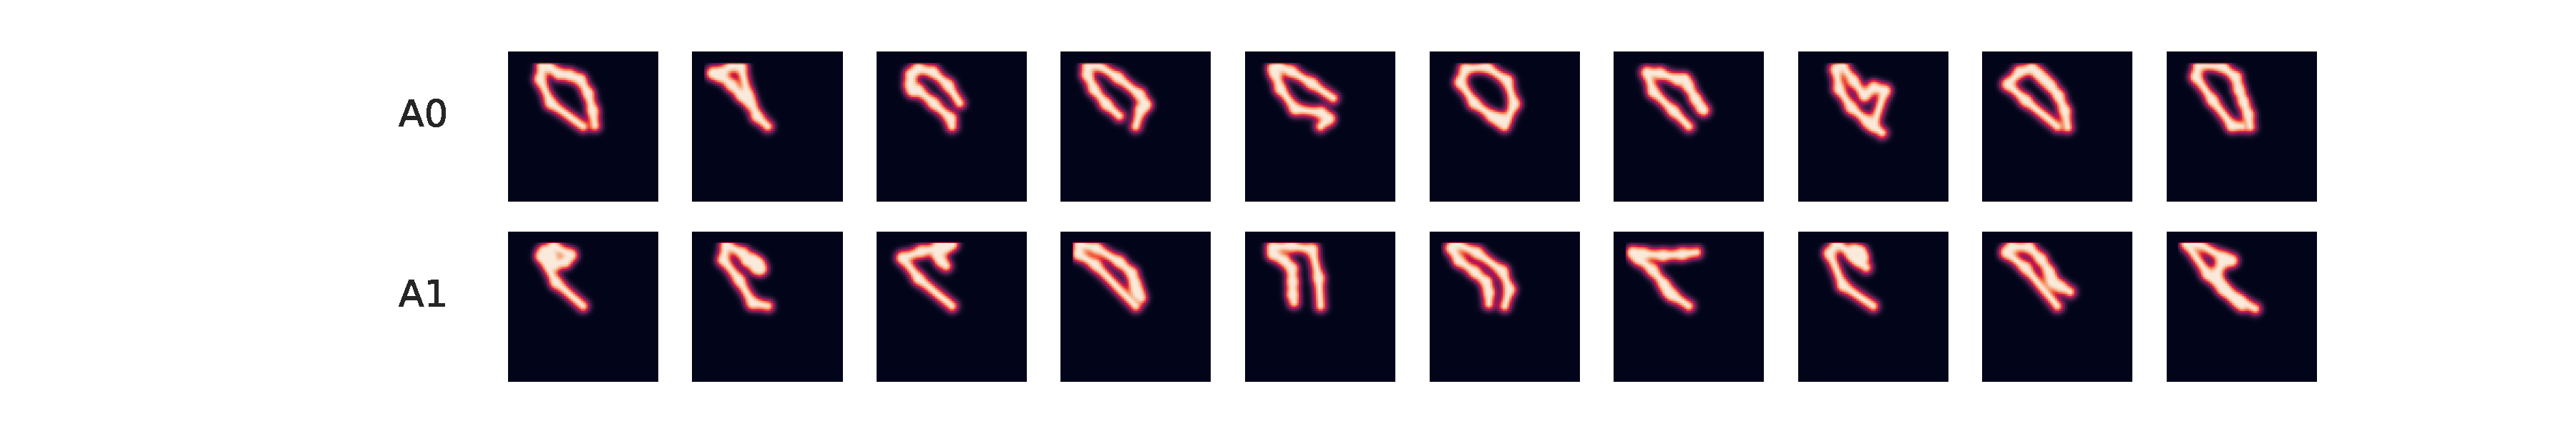
\includegraphics[trim={5cm 1cm 1cm 1cm},clip,width=1\textwidth]{curves/training/Examples_0.pdf}
\caption{Utterances examples for referent 0.}
\end{figure}

\begin{figure}[h!]
\centering
    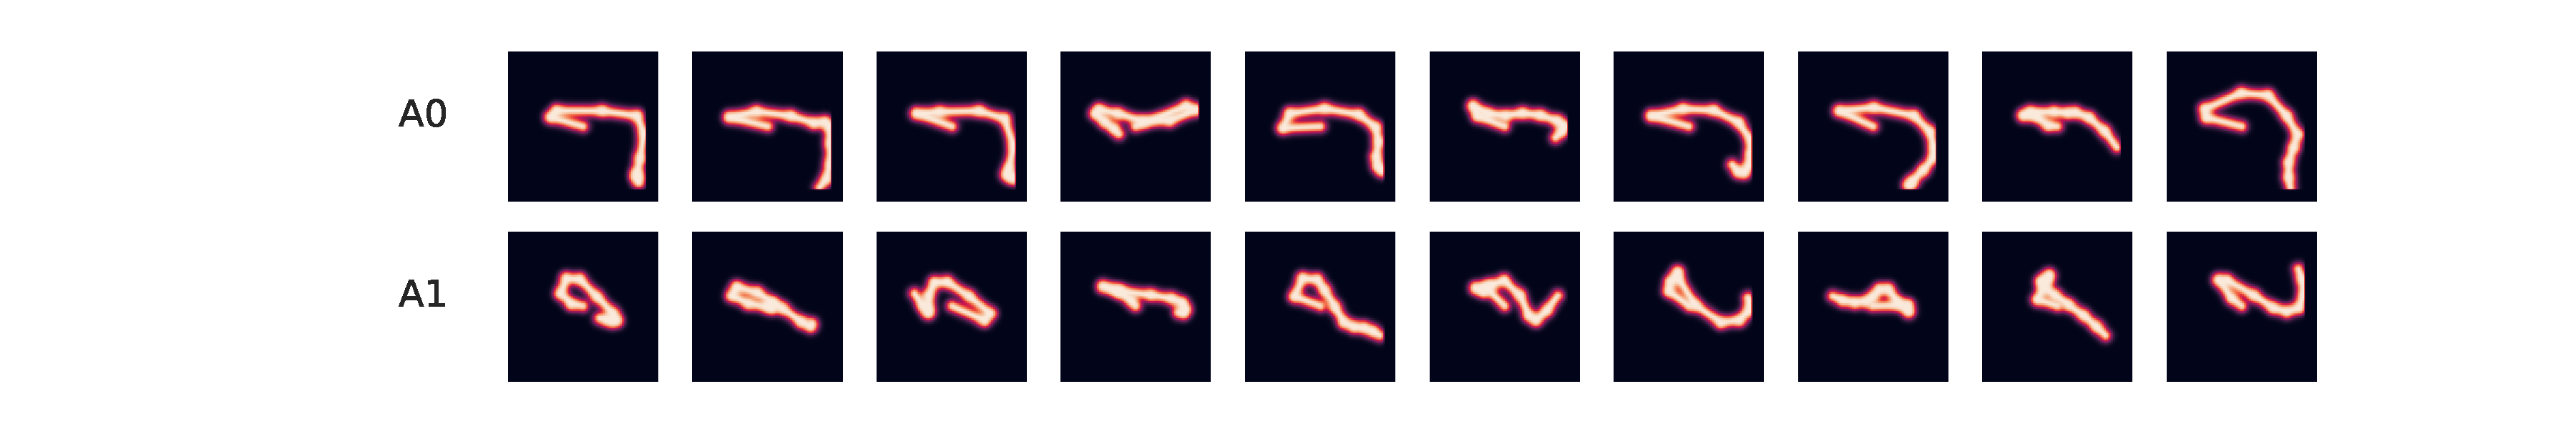
\includegraphics[trim={5cm 1cm 1cm 1cm},clip,width=1\textwidth]{curves/training/Examples_1.pdf}
\caption{Utterances examples for referent 1.}
\end{figure}

\begin{figure}[h!]
\centering
    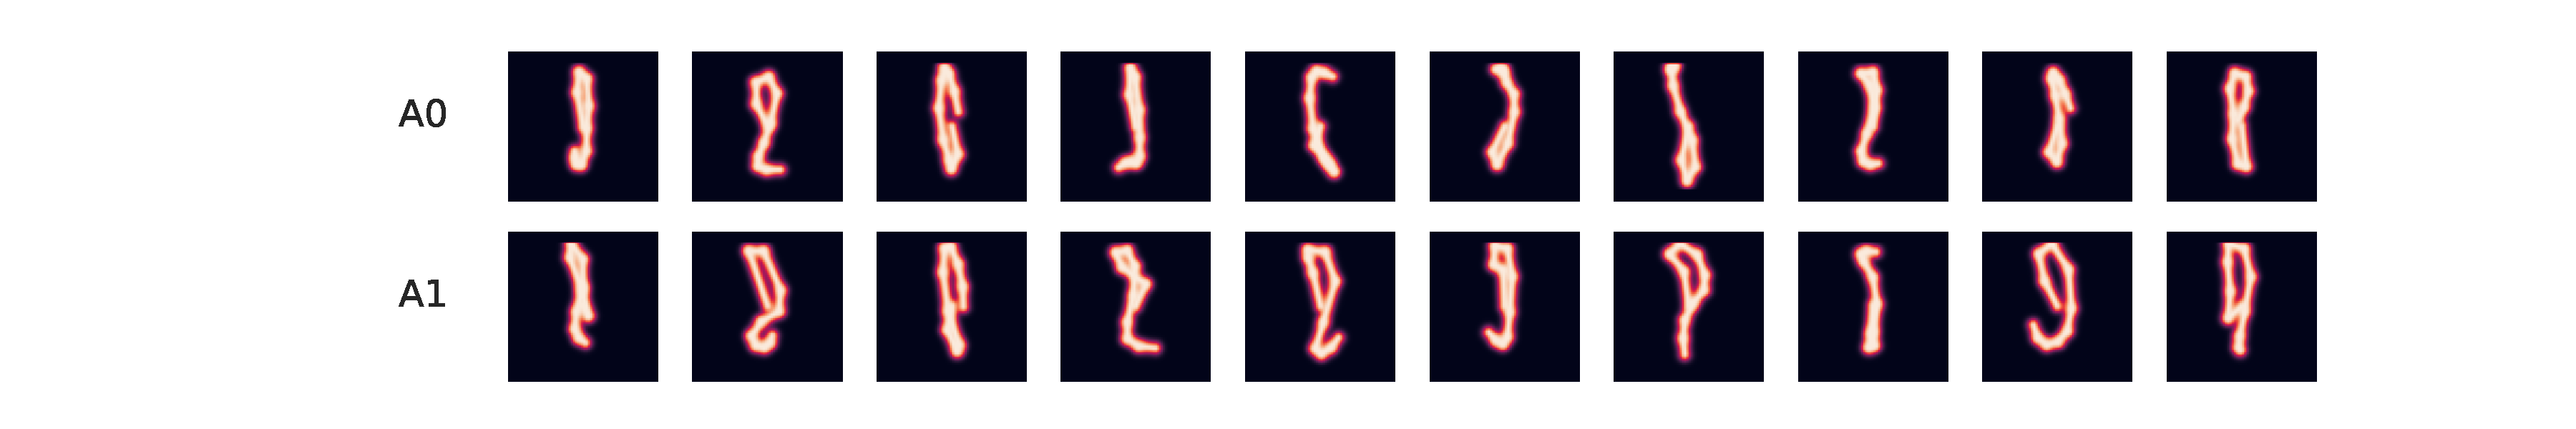
\includegraphics[trim={5cm 1cm 1cm 1cm},clip,width=1\textwidth]{curves/training/Examples_2.pdf}
\caption{Utterances examples for referent 2.}
\end{figure}

\begin{figure}[h!]
\centering
    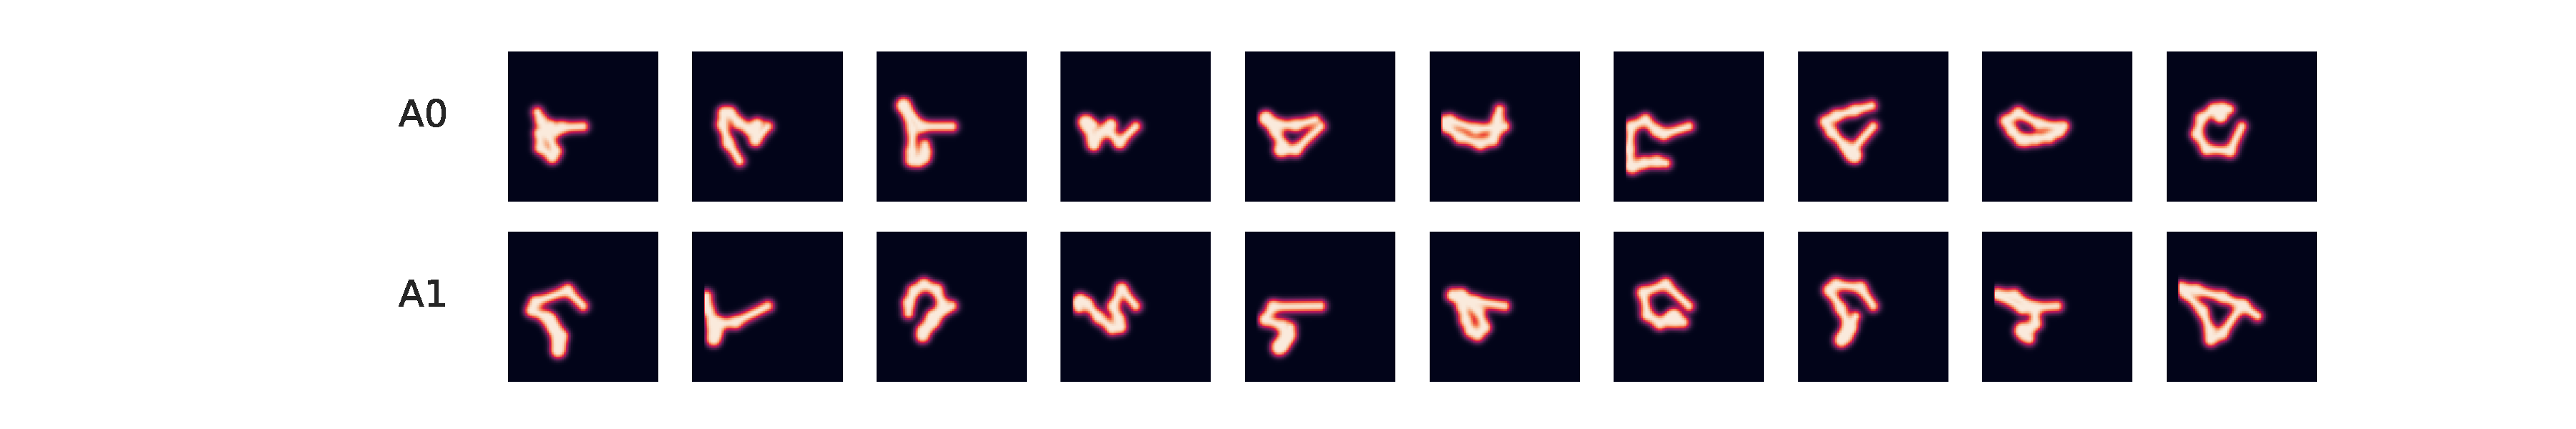
\includegraphics[trim={5cm 1cm 1cm 1cm},clip,width=1\textwidth]{curves/training/Examples_3.pdf}
\caption{Utterances examples for referent 3.}
\end{figure}

\begin{figure}[h!]
\centering
    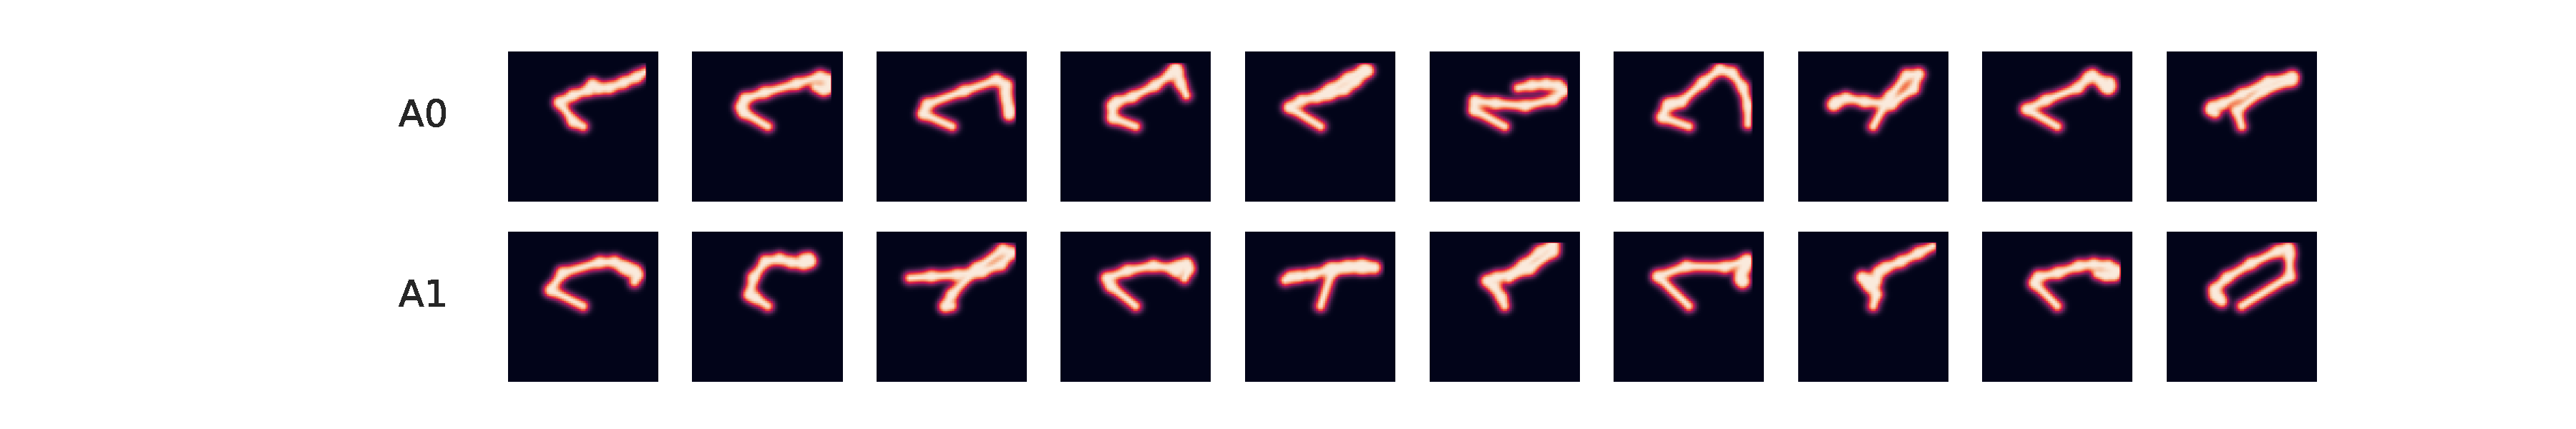
\includegraphics[trim={5cm 1cm 1cm 1cm},clip,width=1\textwidth]{curves/training/Examples_4.pdf}
\caption{Utterances examples for referent 4.}
\end{figure}

\newpage
\subsection{Topographic Maps \& Scores}
\label{sup:topo_maps}

\subsubsection{One-Hot}

\begin{figure}[!h]
    \centering
     \begin{tabular}{ccc}

     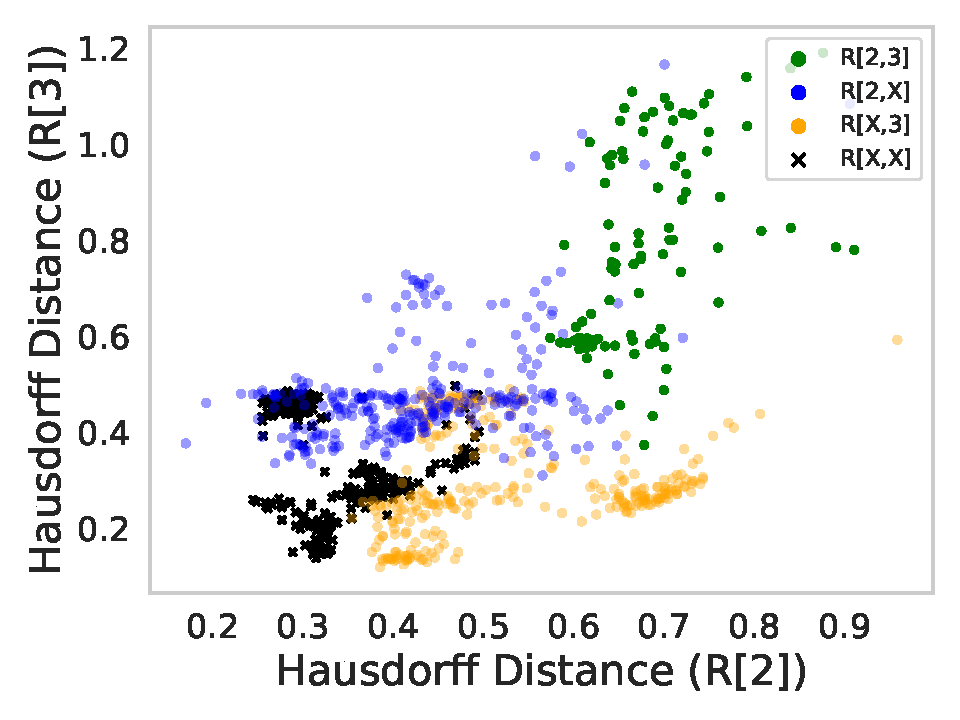
\includegraphics[width=0.3\textwidth]{curves/onehot_distance_plots/0_d=-0.401.pdf} & 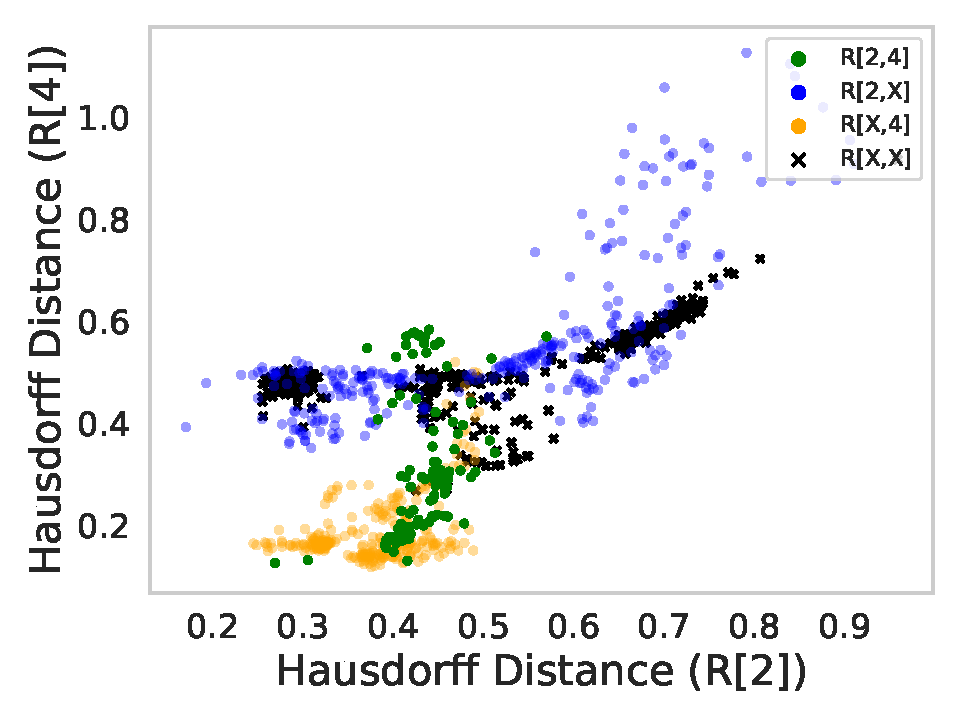
\includegraphics[width=0.3\textwidth]{curves/onehot_distance_plots/1_d=-0.111.pdf} &  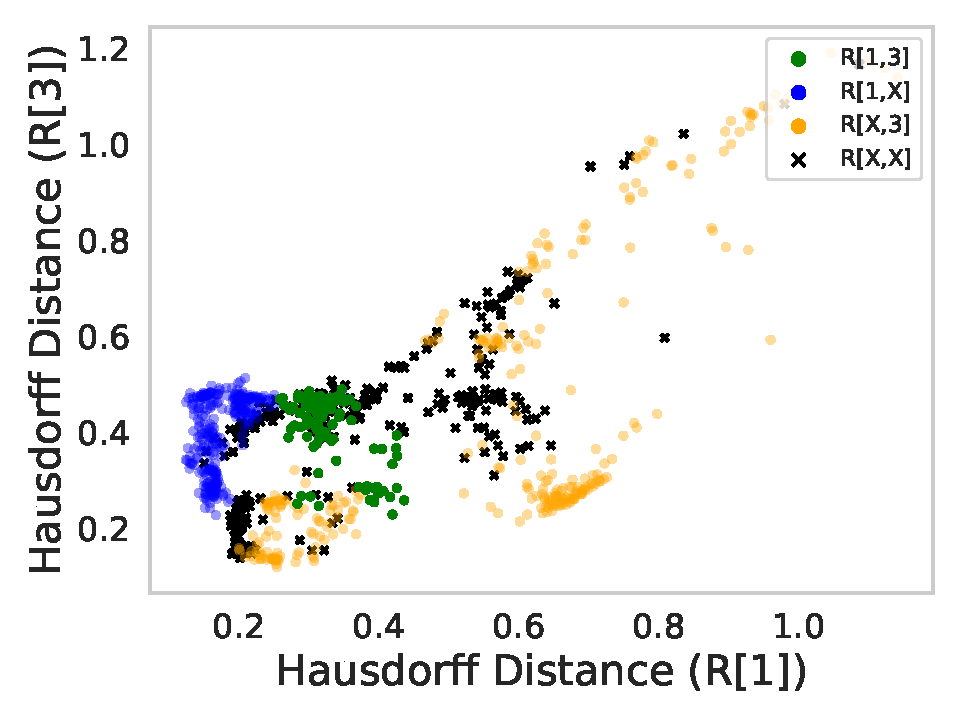
\includegraphics[width=0.3\textwidth]{curves/onehot_distance_plots/2_d=-0.085.pdf}    \\
     $\rho=-0.401$ & $\rho=-0.111$ & $\rho=-0.085$                                                                \\
     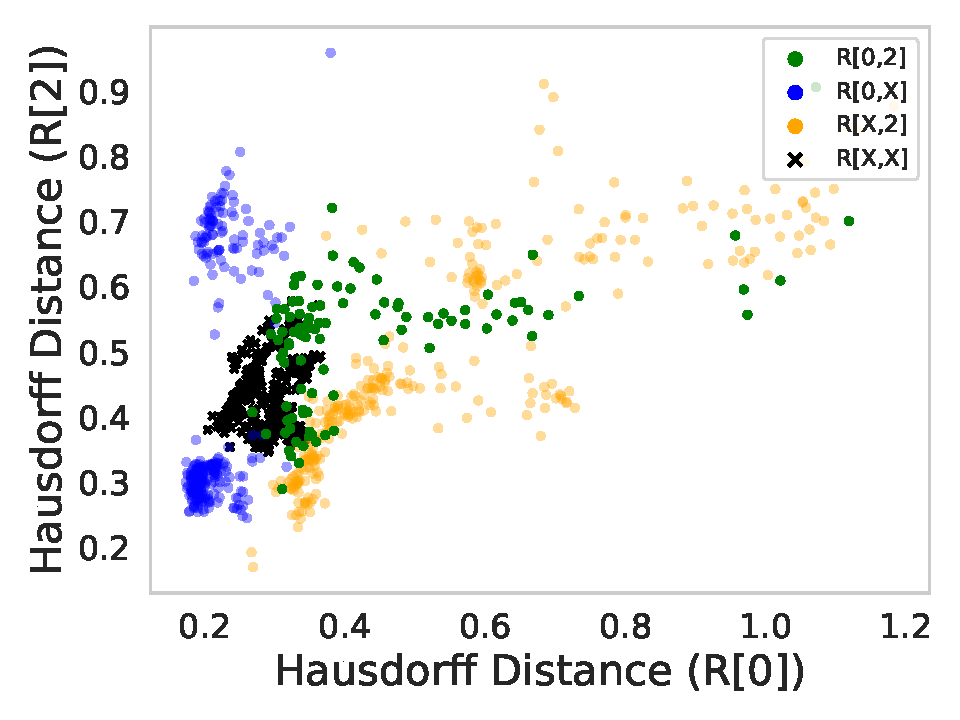
\includegraphics[width=0.3\textwidth]{curves/onehot_distance_plots/3_d=0.041.pdf} & 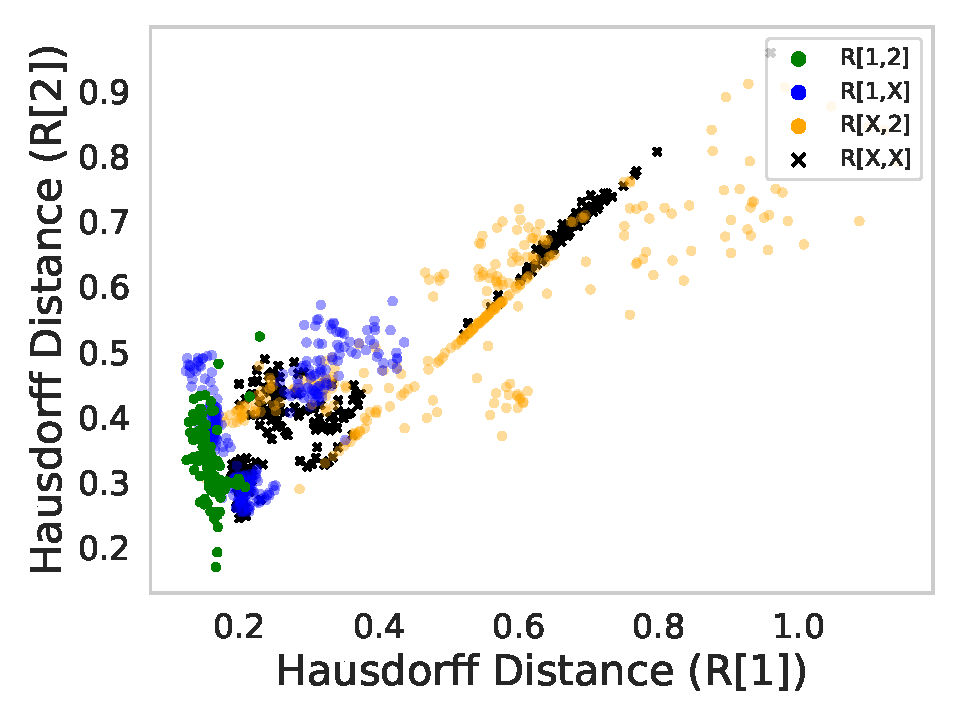
\includegraphics[width=0.3\textwidth]{curves/onehot_distance_plots/4_d=0.09.pdf} &  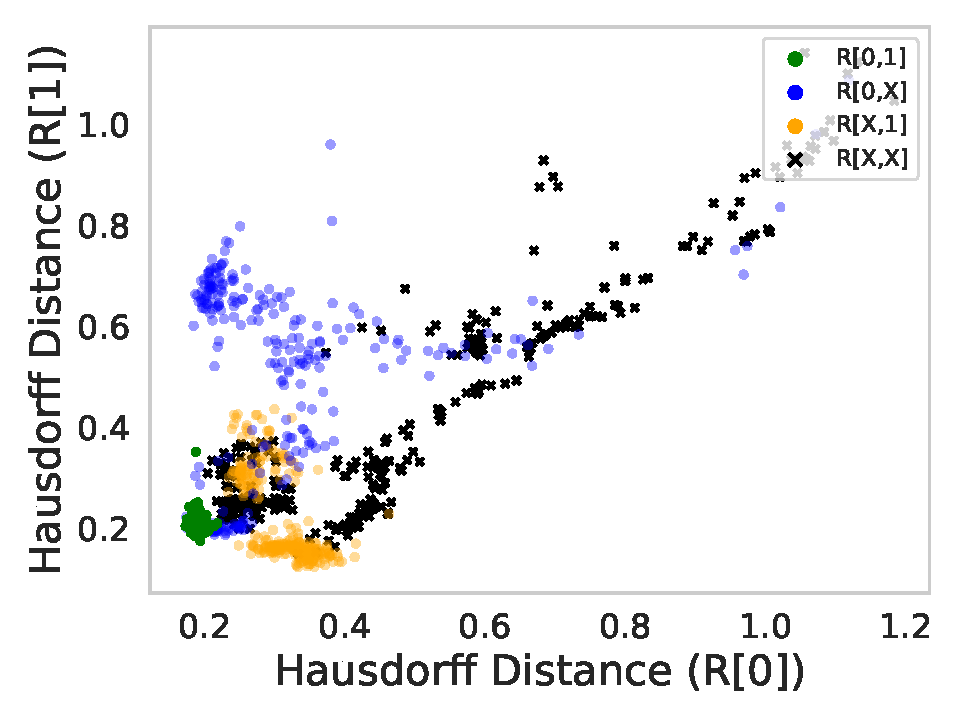
\includegraphics[width=0.3\textwidth]{curves/onehot_distance_plots/5_d=0.094.pdf}    \\
     $\rho=0.041$ & $\rho=0.09$ & $\rho=0.094$                                                                              \\
     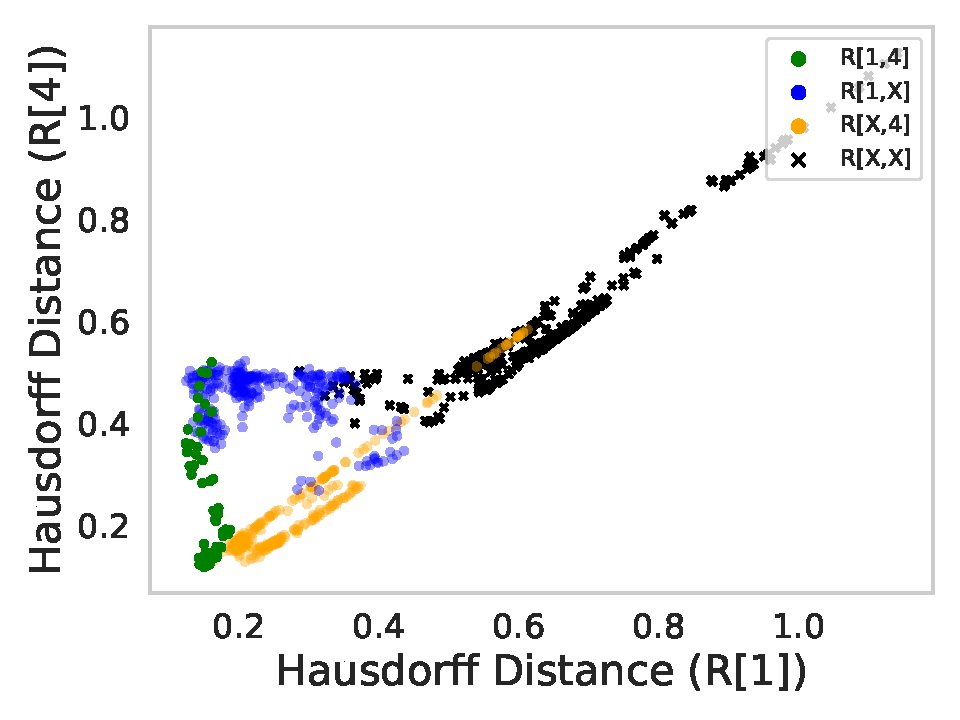
\includegraphics[width=0.3\textwidth]{curves/onehot_distance_plots/6_d=0.1.pdf} & 
     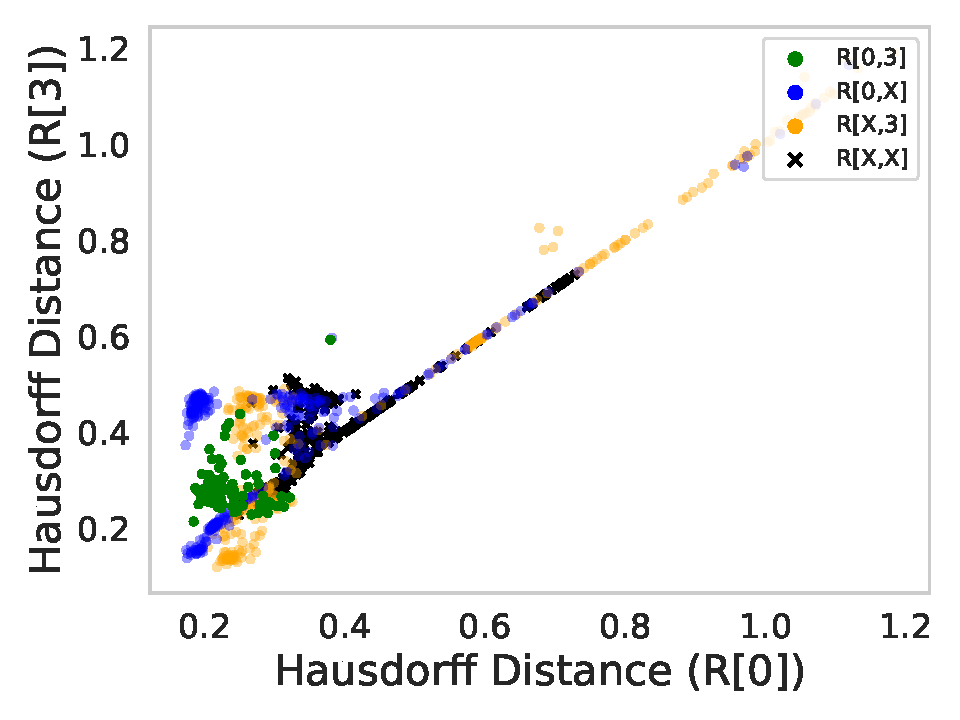
\includegraphics[width=0.3\textwidth]{curves/onehot_distance_plots/7_d=0.114.pdf} &  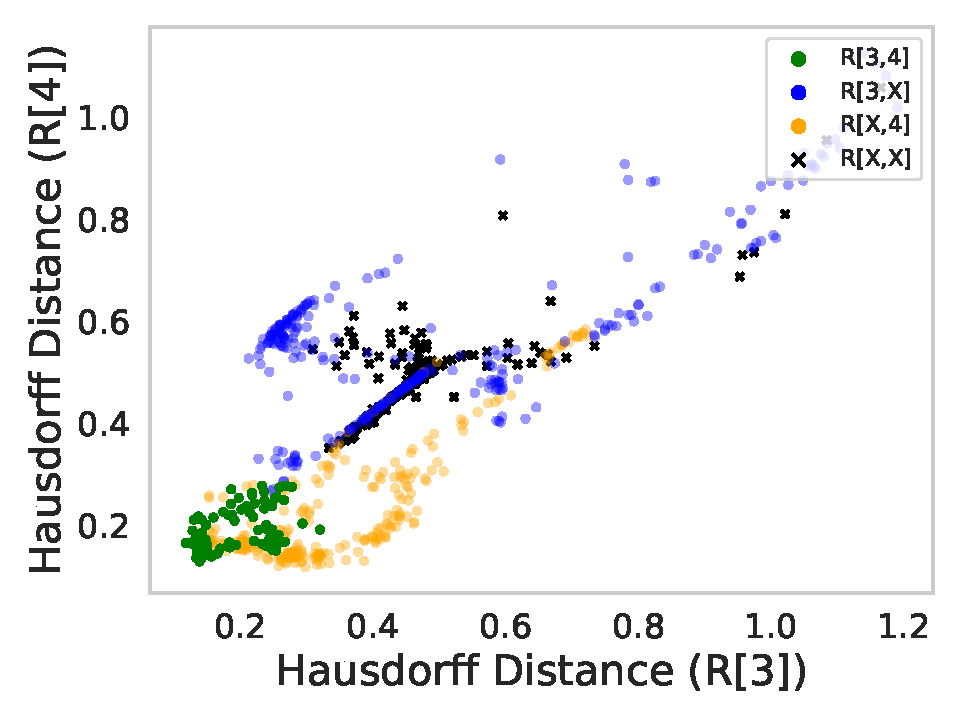
\includegraphics[width=0.3\textwidth]{curves/onehot_distance_plots/8_d=0.133.pdf}    \\
     $\rho=0.1$ & $\rho=0.114$ & $\rho=0.133$                                                                           \\
     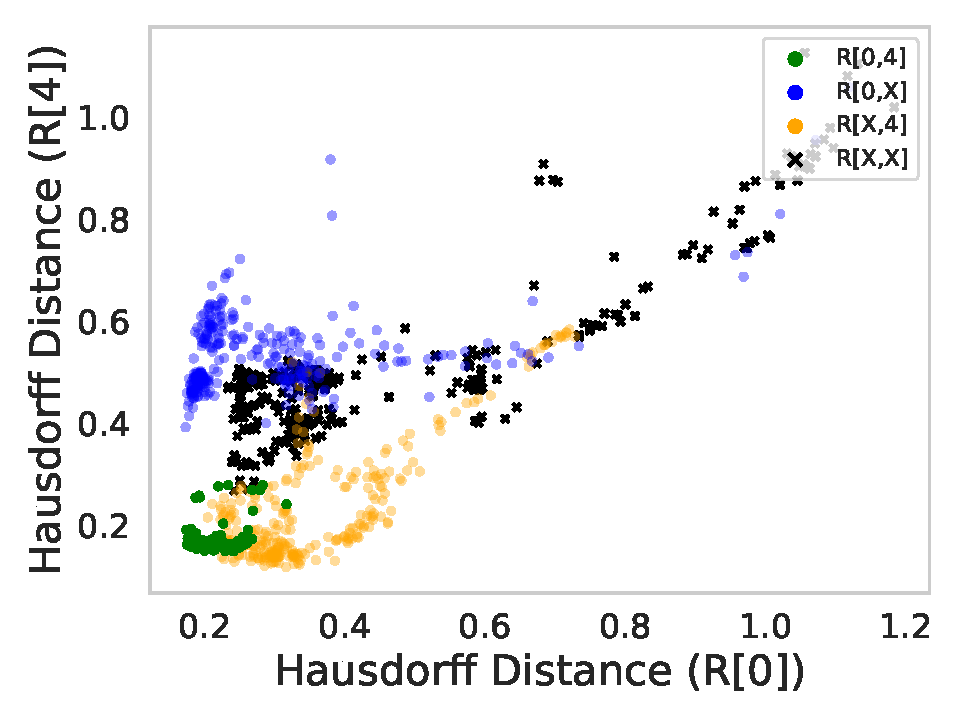
\includegraphics[width=0.3\textwidth]{curves/onehot_distance_plots/9_d=0.147.pdf} & &    \\
     $\rho=0.147$ &  &                                                                                   \\
    
 \end{tabular}
    \caption{Topographic maps and their associated topographic scores for each combination of features with one-hot referents}
    \label{fig:sup_topo_one_hot}
\end{figure}


\newpage

\subsubsection{Visual - Shared Perspectives}

\begin{figure}[!h]
 \begin{tabular}{ccc}

     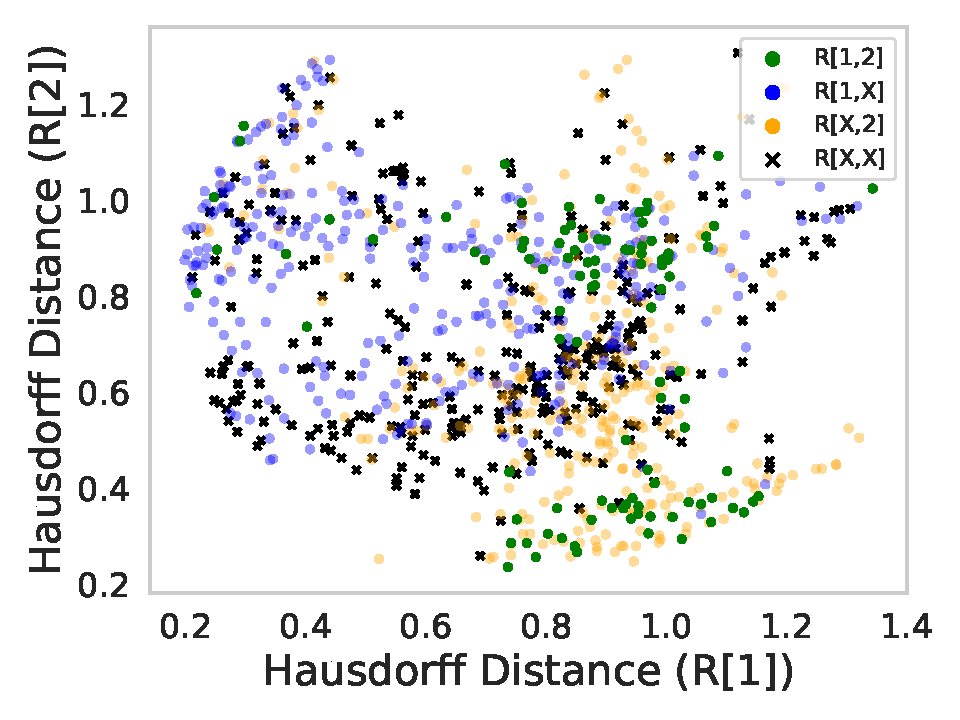
\includegraphics[width=0.3\textwidth]{curves/shared_distance_plots/0_d=-0.047.pdf} & 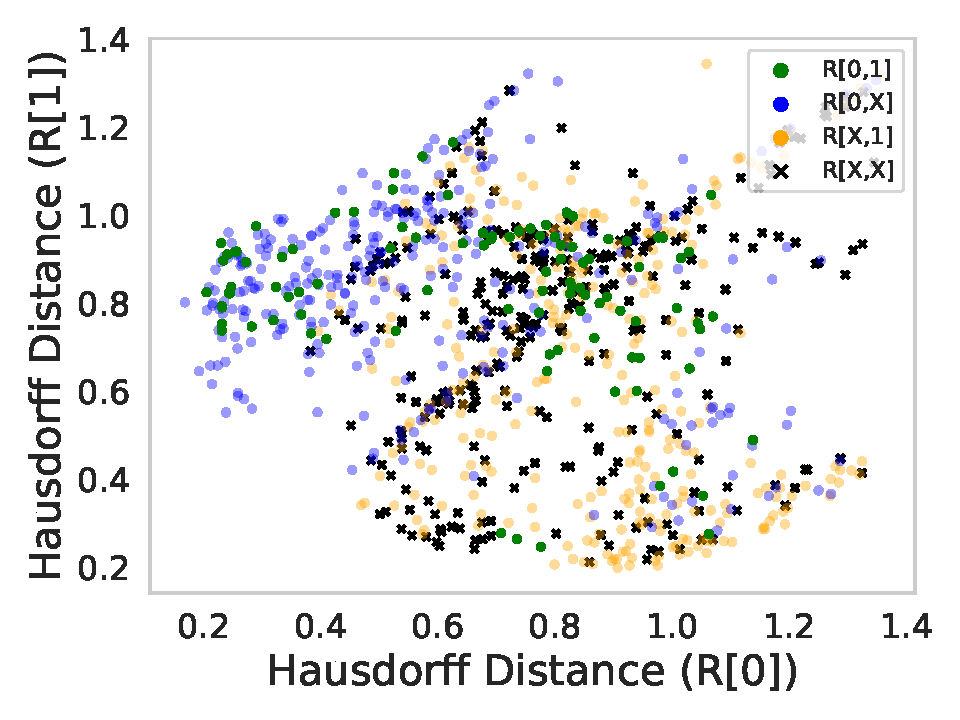
\includegraphics[width=0.3\textwidth]{curves/shared_distance_plots/1_d=-0.044.pdf} &  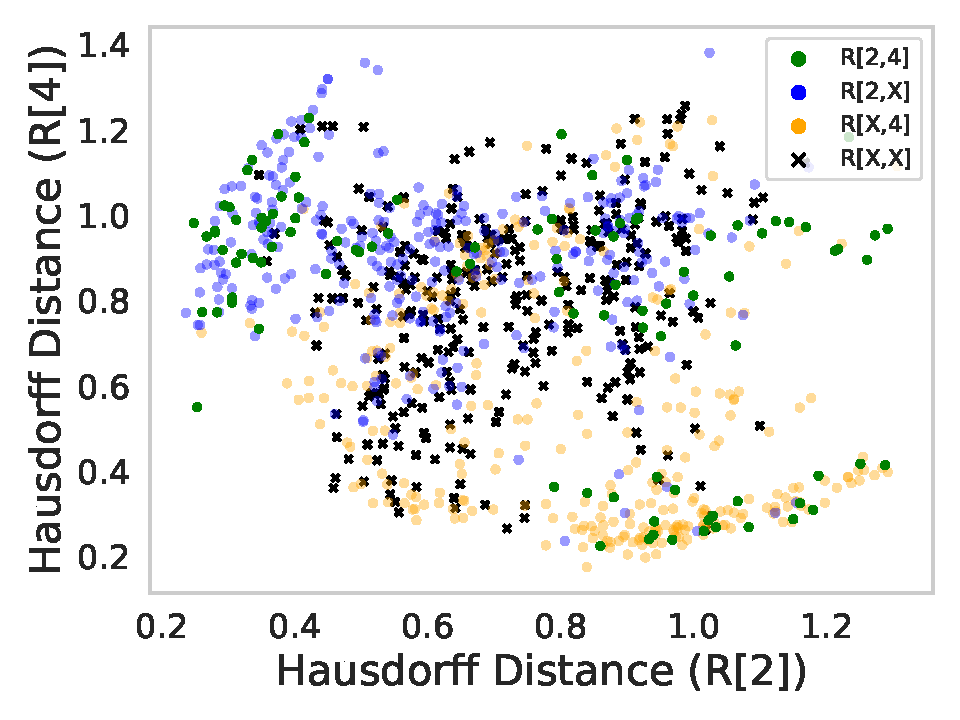
\includegraphics[width=0.3\textwidth]{curves/shared_distance_plots/2_d=0.005.pdf}    \\
     $\rho=-0.047$ & $\rho=-0.044$ & $\rho=0.005$                                                                \\
     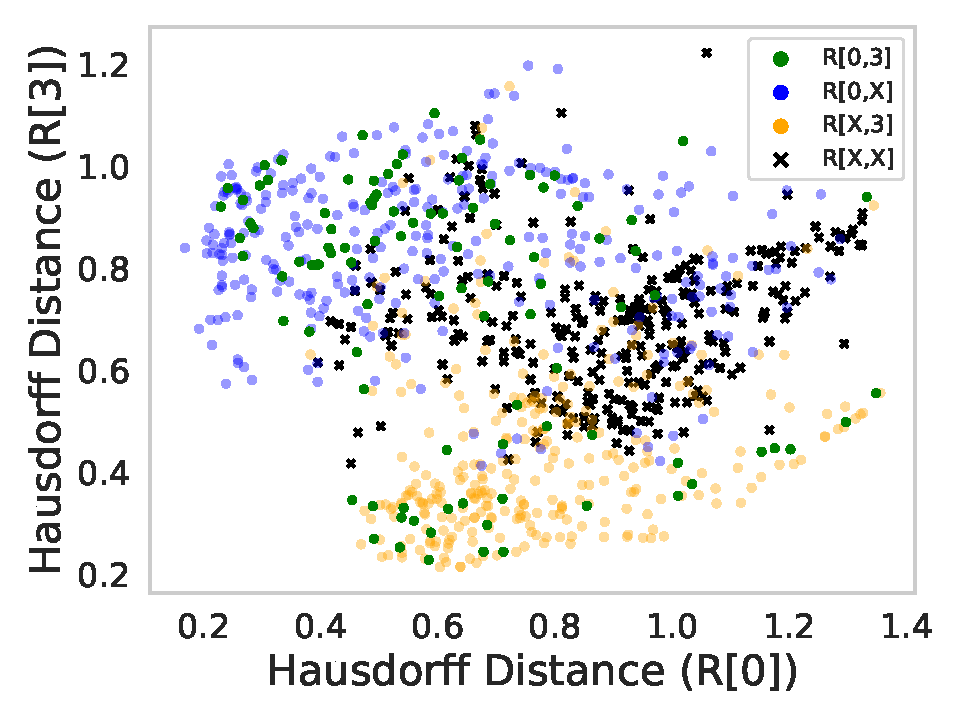
\includegraphics[width=0.3\textwidth]{curves/shared_distance_plots/3_d=0.073.pdf} & 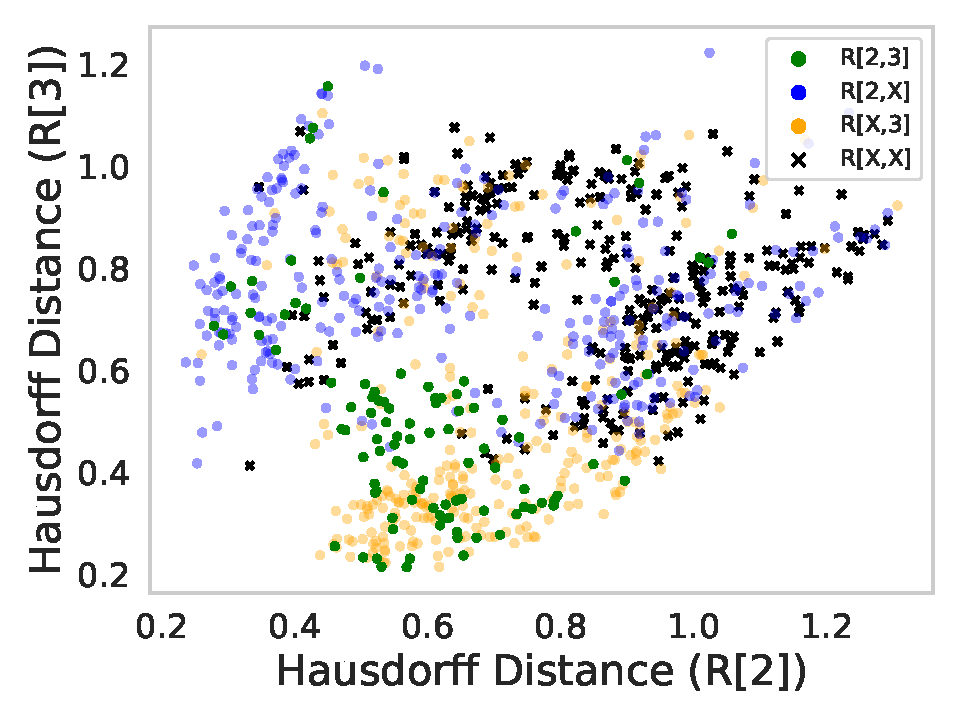
\includegraphics[width=0.3\textwidth]{curves/shared_distance_plots/4_d=0.081.pdf} &  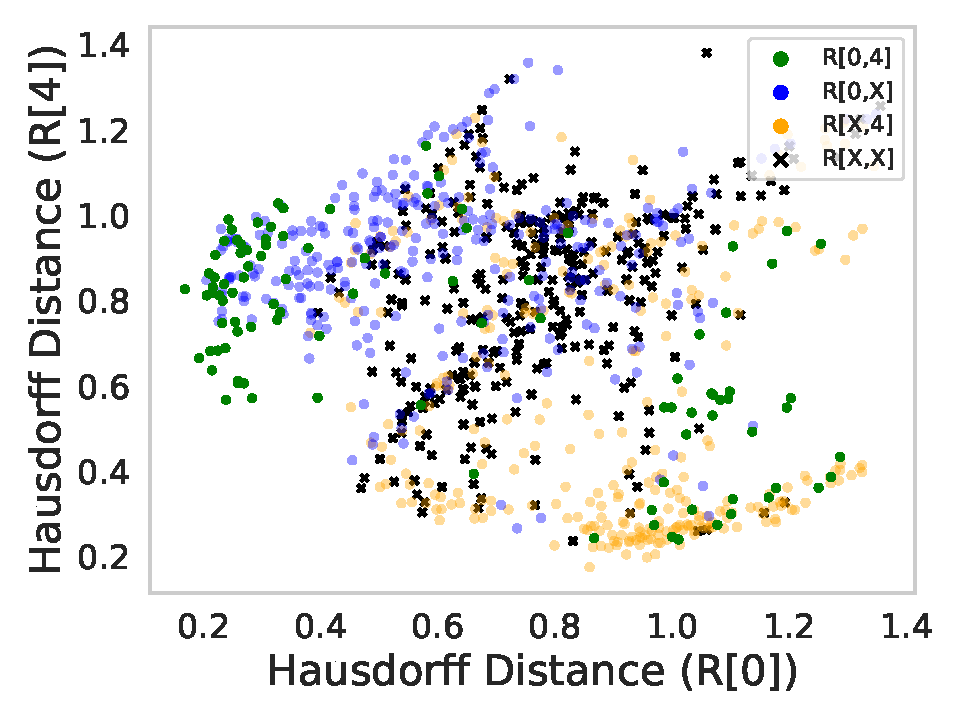
\includegraphics[width=0.3\textwidth]{curves/shared_distance_plots/5_d=0.137.pdf}    \\
     $\rho=0.073$ & $\rho=0.081$ & $\rho=0.137$                                                                             \\
     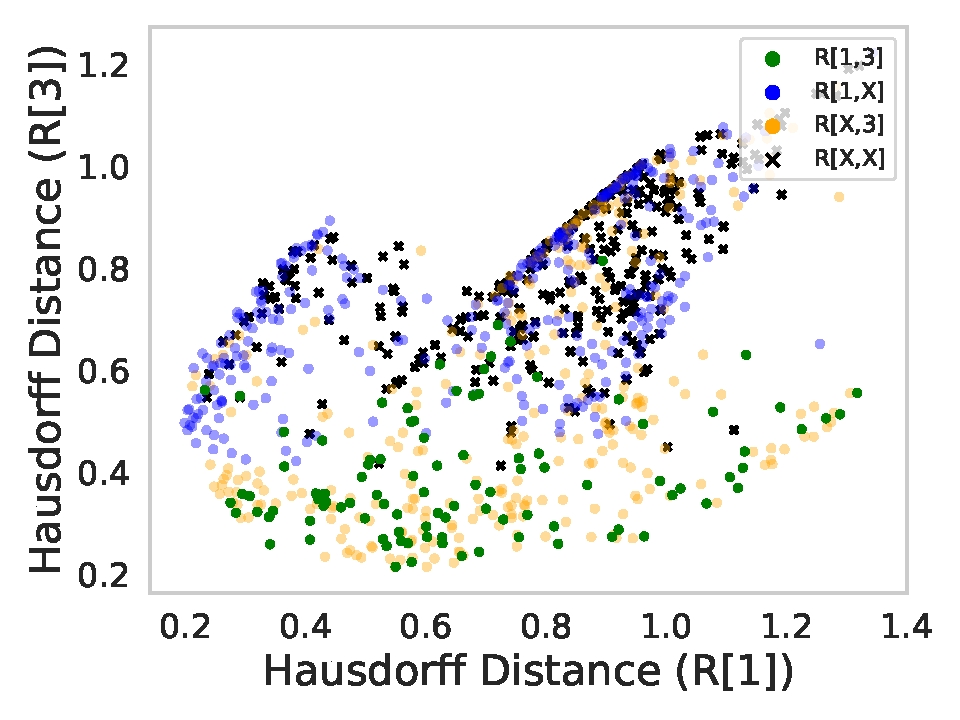
\includegraphics[width=0.3\textwidth]{curves/shared_distance_plots/6_d=0.16.pdf} & 
     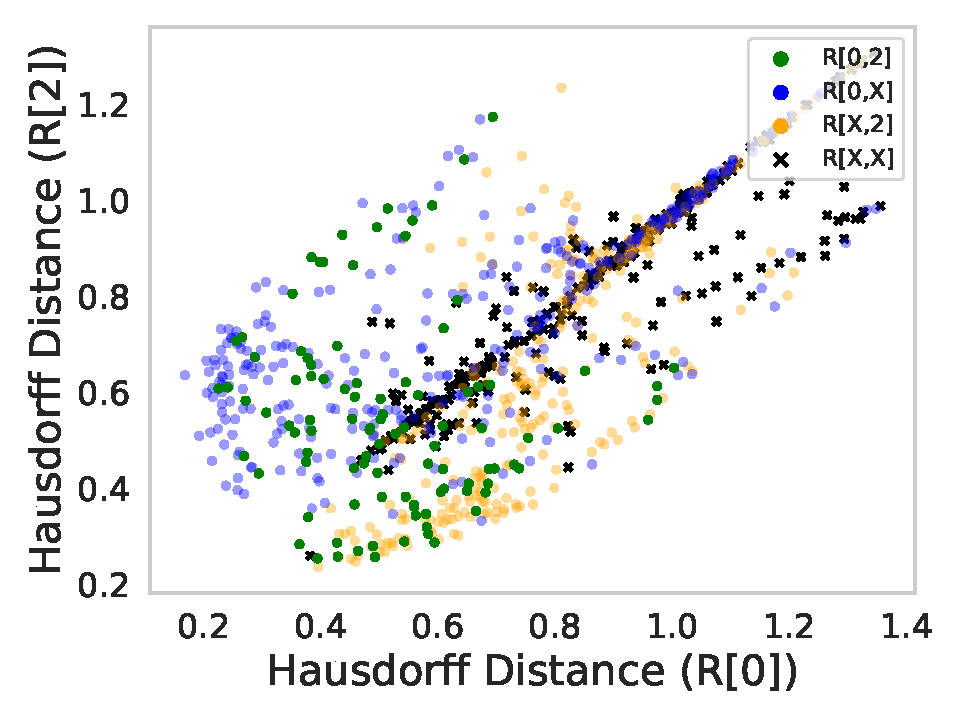
\includegraphics[width=0.3\textwidth]{curves/shared_distance_plots/7_d=0.215.pdf} &  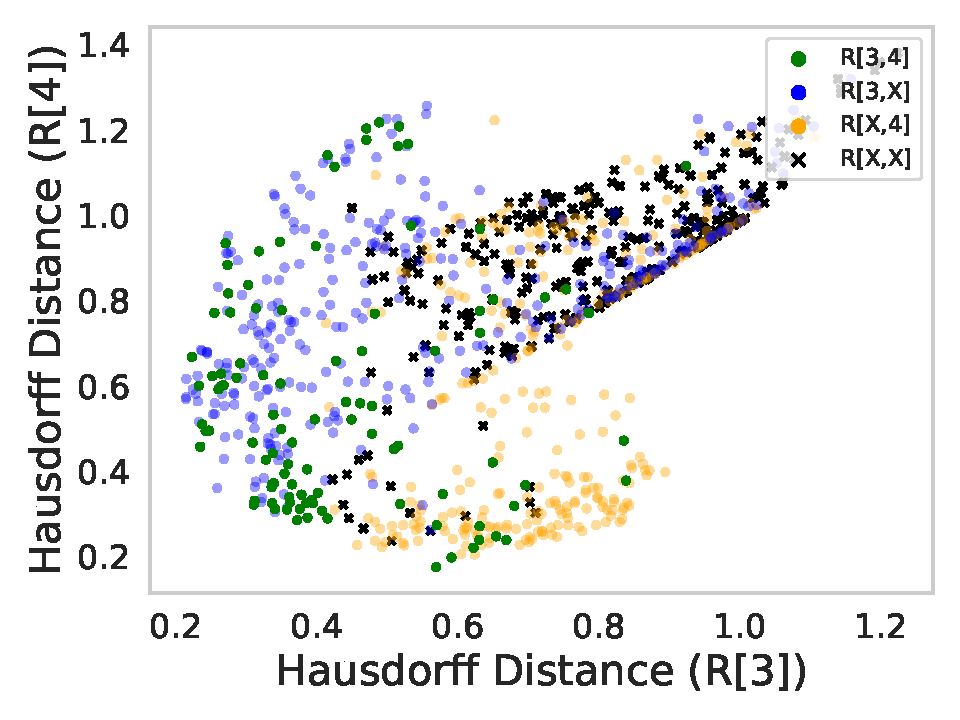
\includegraphics[width=0.3\textwidth]{curves/shared_distance_plots/8_d=0.242.pdf}    \\
     $\rho=0.16$ & $\rho=0.215$ & $\rho=0.242$                                                                              \\
     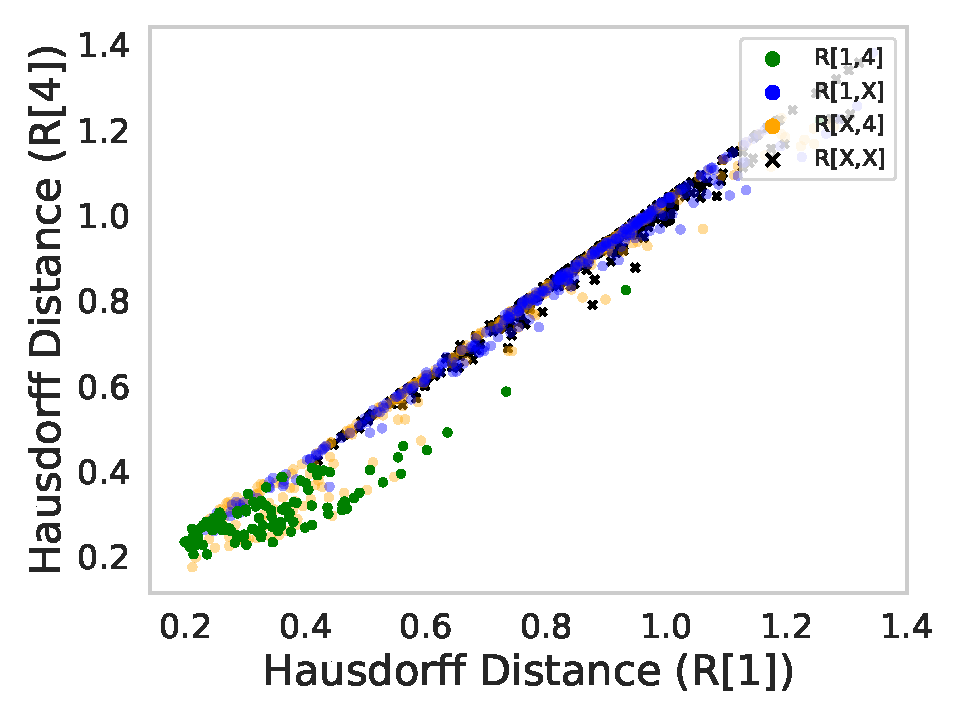
\includegraphics[width=0.3\textwidth]{curves/shared_distance_plots/9_d=0.501.pdf} & &    \\
     $\rho=0.501$ &  &                                                                                   \\
    
 \end{tabular}
     \caption{Topographic maps and their associated topographic scores for each combination of features with shared-visual referents}
\label{fig:sup_topo_shared}
\end{figure}


\newpage

\subsubsection{Visual - Unshared Perspectives}

\begin{figure}[!h]
    \centering
 \begin{tabular}{ccc}

     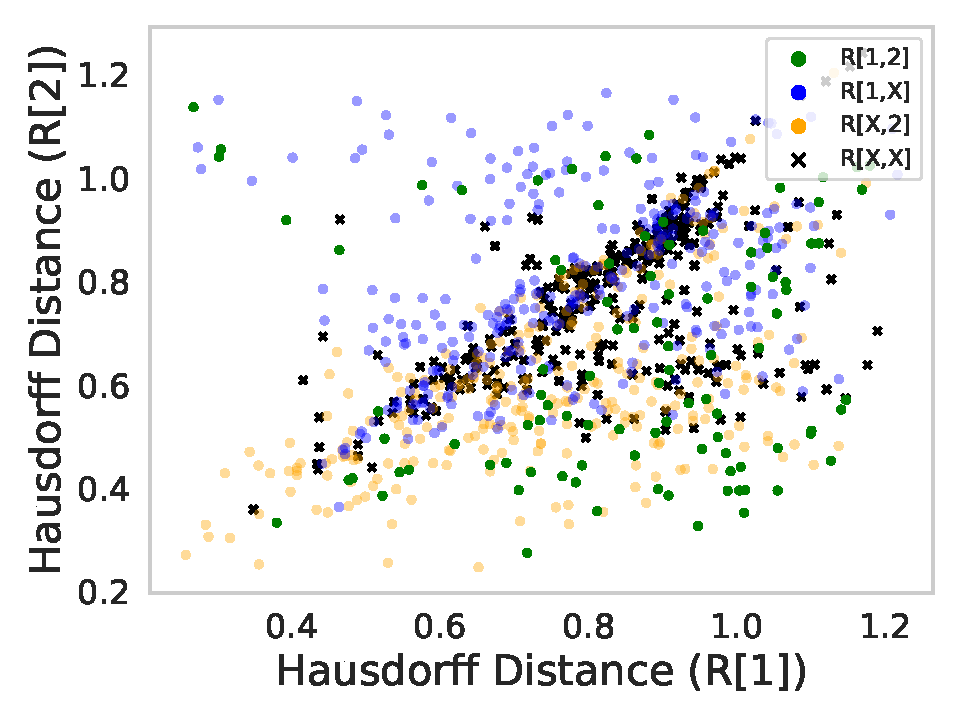
\includegraphics[width=0.3\textwidth]{curves/unshared_distance_plots/0_d=-0.113.pdf} & 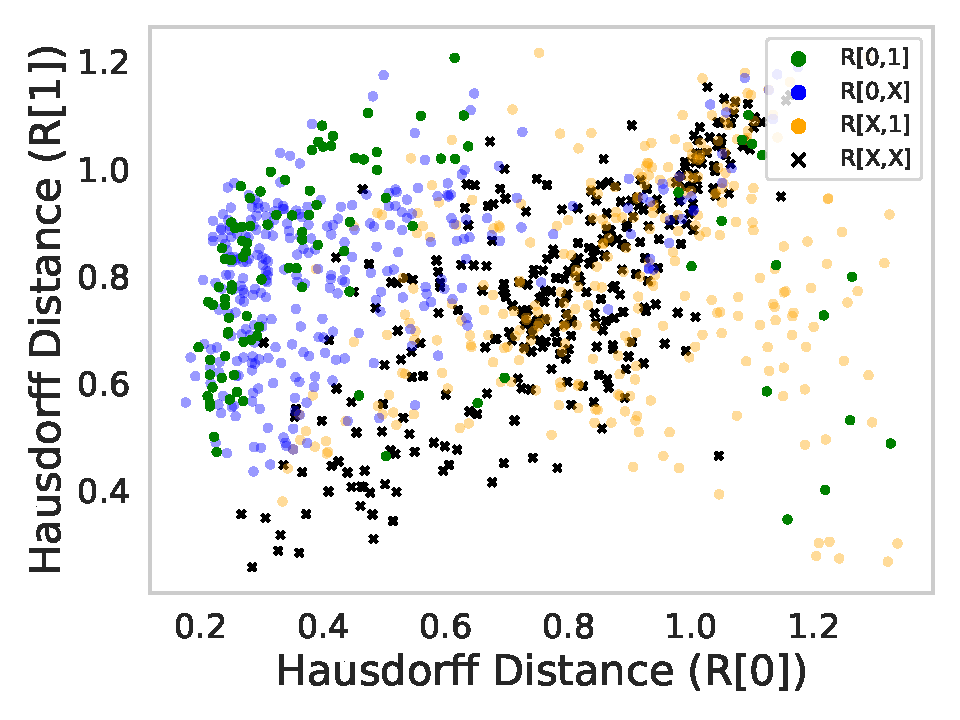
\includegraphics[width=0.3\textwidth]{curves/unshared_distance_plots/1_d=-0.016.pdf} &  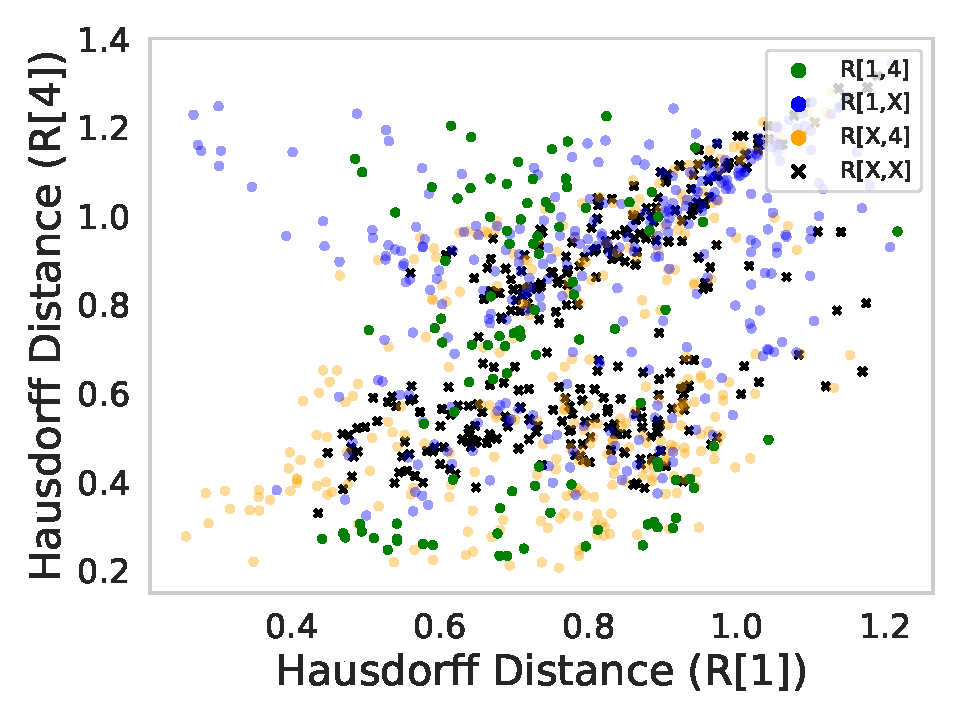
\includegraphics[width=0.3\textwidth]{curves/unshared_distance_plots/2_d=0.007.pdf}    \\
     $\rho=-0.113$ & $\rho=-0.016$ & $\rho=0$                                                                \\
     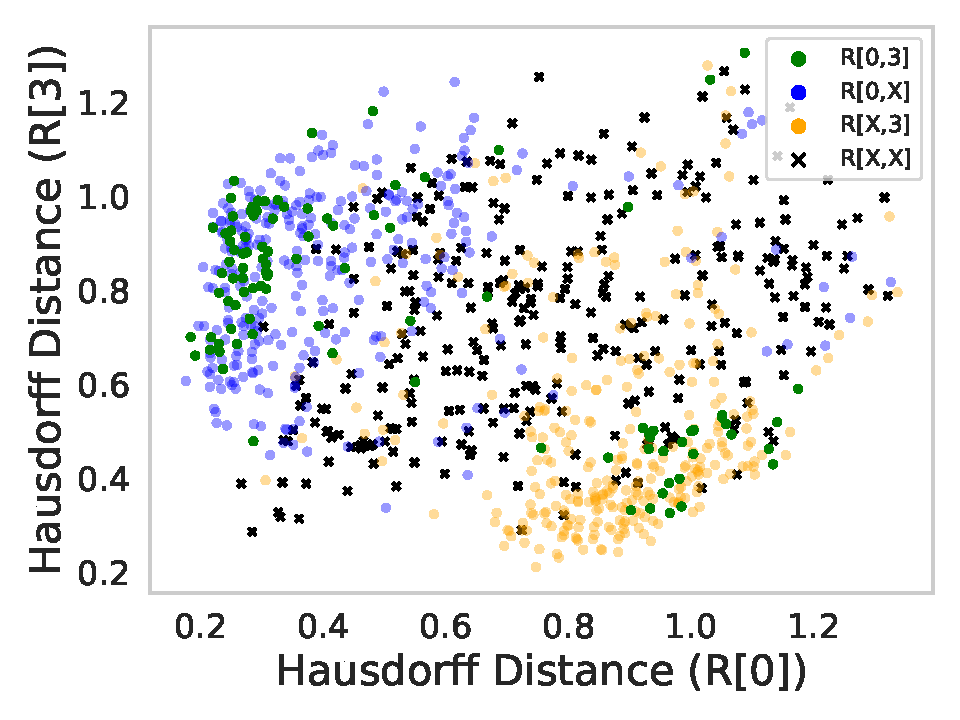
\includegraphics[width=0.3\textwidth]{curves/unshared_distance_plots/3_d=0.019.pdf} & 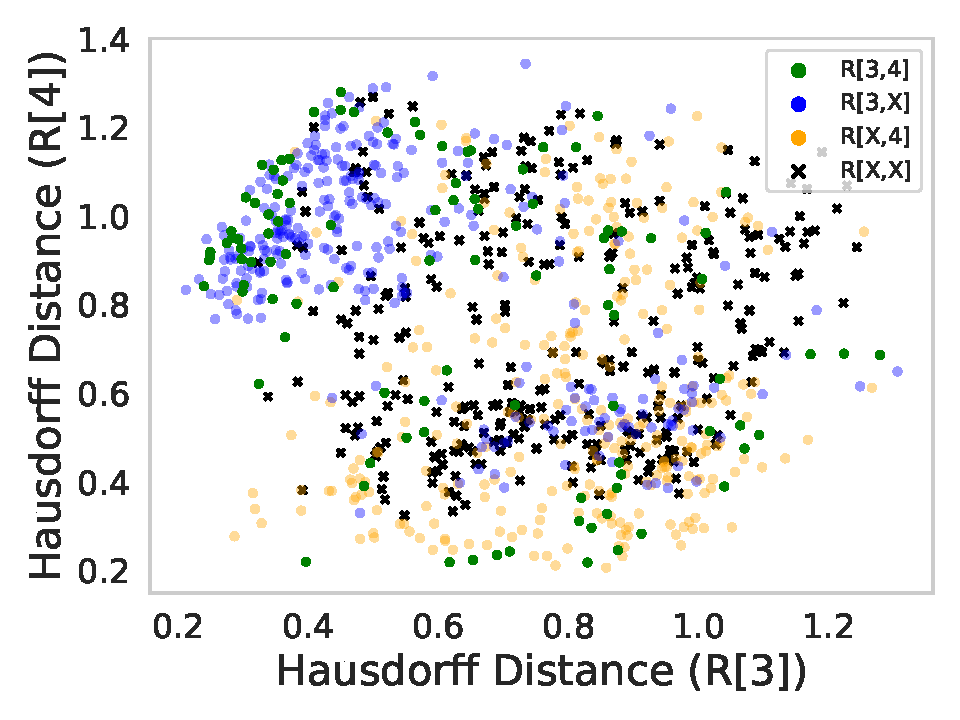
\includegraphics[width=0.3\textwidth]{curves/unshared_distance_plots/4_d=0.026.pdf} &  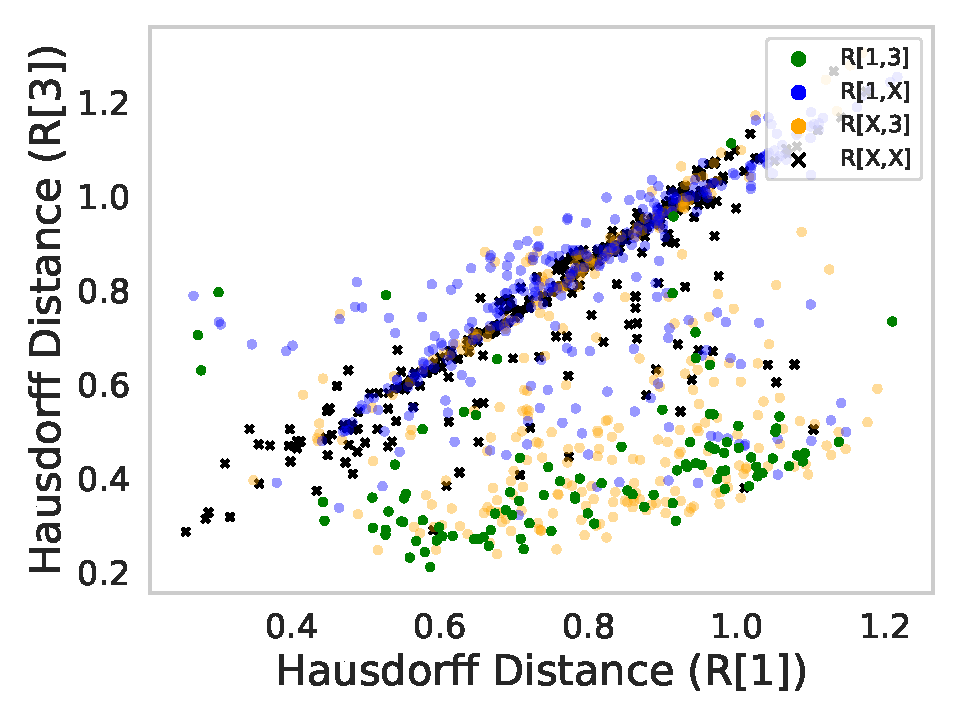
\includegraphics[width=0.3\textwidth]{curves/unshared_distance_plots/5_d=0.13.pdf}    \\
     $\rho=0.019$ & $\rho=0.026$ & $\rho=0.13$                                                                              \\
     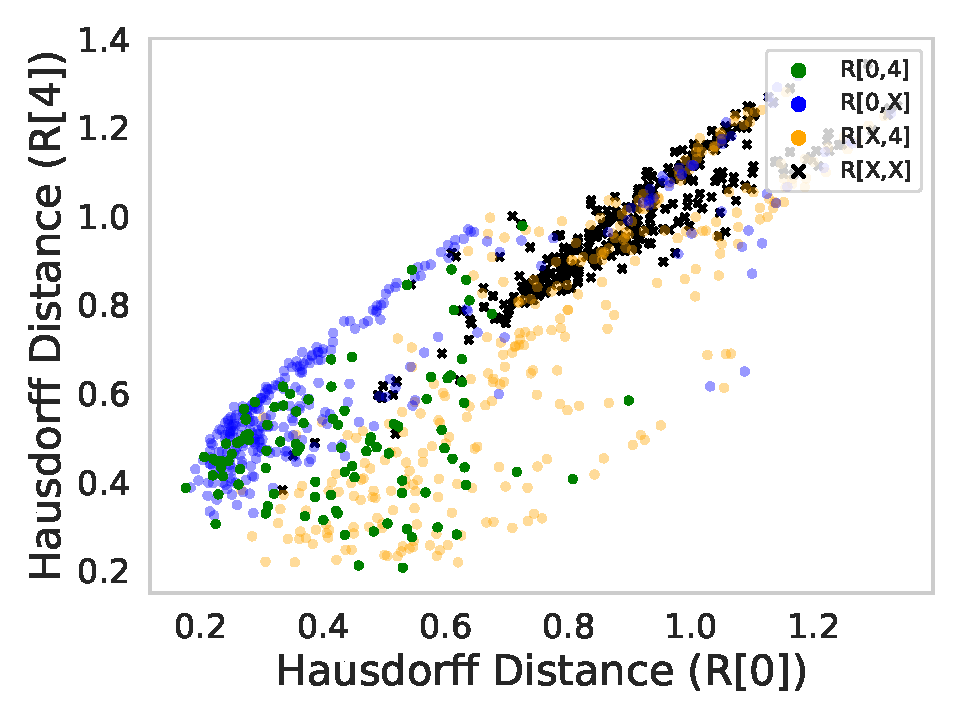
\includegraphics[width=0.3\textwidth]{curves/unshared_distance_plots/6_d=0.137.pdf} & 
     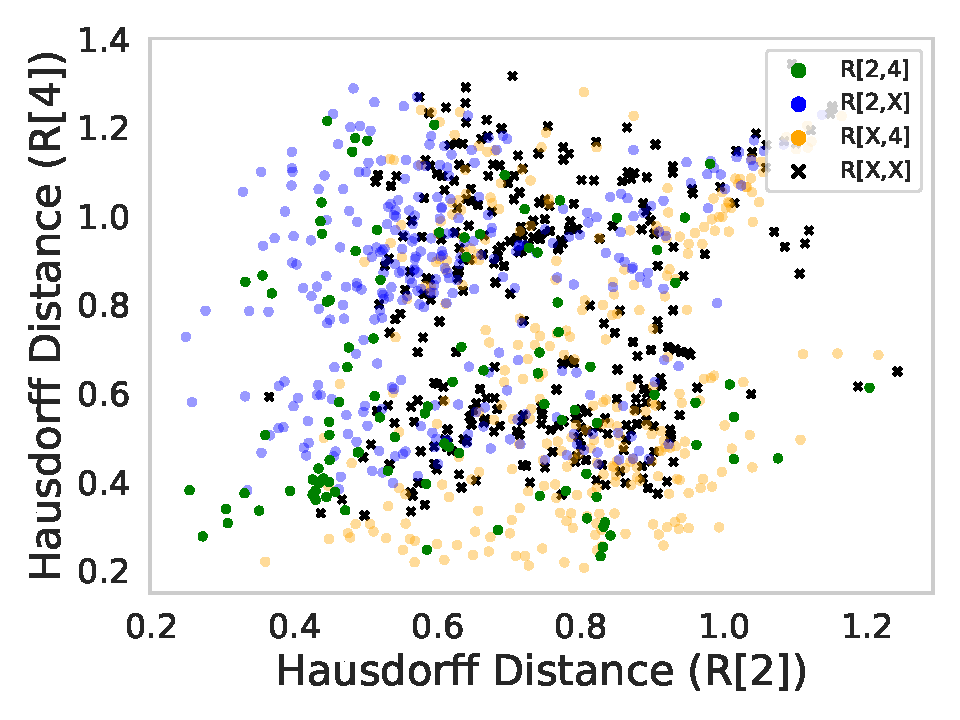
\includegraphics[width=0.3\textwidth]{curves/unshared_distance_plots/7_d=0.156.pdf} &  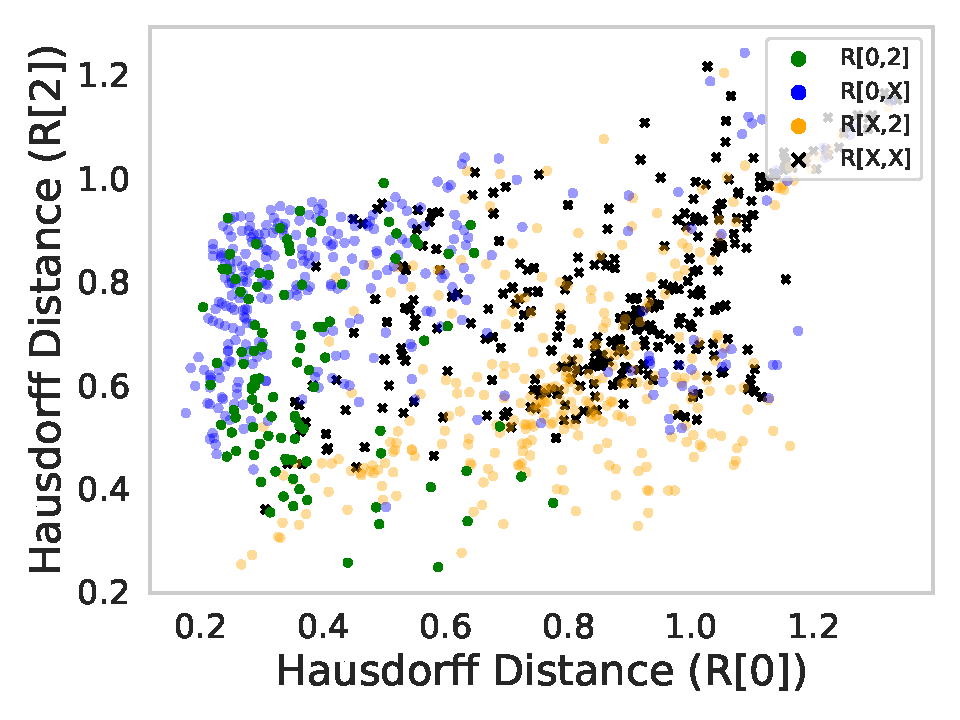
\includegraphics[width=0.3\textwidth]{curves/unshared_distance_plots/8_d=0.18.pdf}    \\
     $\rho=0.137$ & $\rho=0.156$ & $\rho=0.18$                                                                              \\
     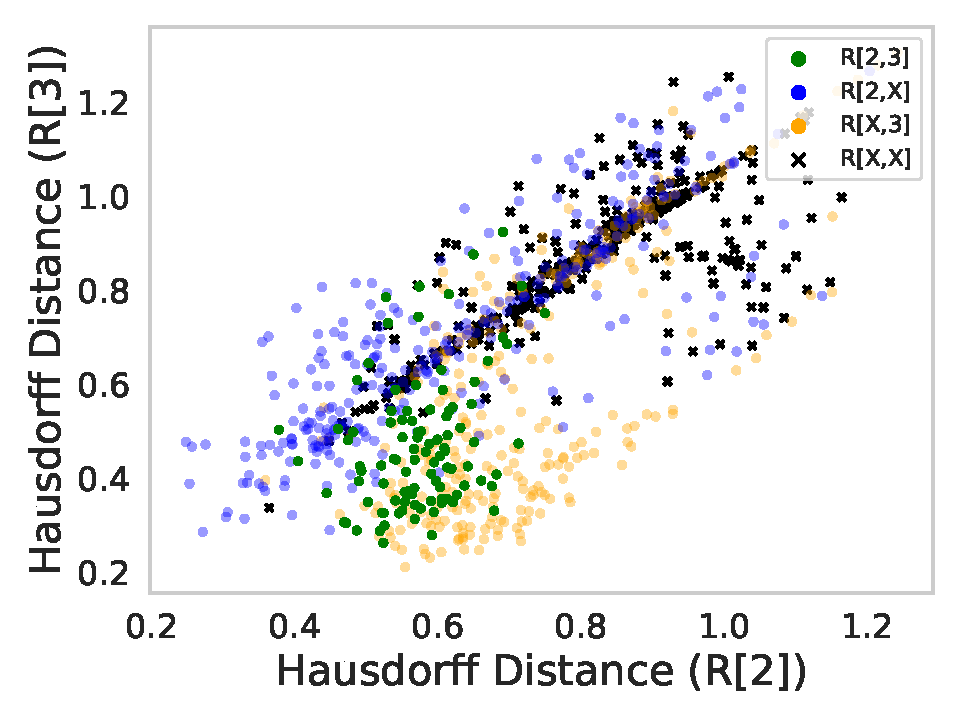
\includegraphics[width=0.3\textwidth]{curves/unshared_distance_plots/9_d=0.203.pdf} & &    \\
     $\rho=0.203$ &  &                                                                                   \\
    
 \end{tabular}
 
      \caption{Topographic maps and their associated topographic scores for each combination of features with unshared-visual referents}
\label{fig:sup_topo_unshared}
\end{figure}

\newpage

\subsection{Composition Matrix examples (Visual - Unshared Perspectives)}
\label{sup:compo_matr}
\begin{figure}[h!]
\centering 

 \begin{tabular}{cc}

     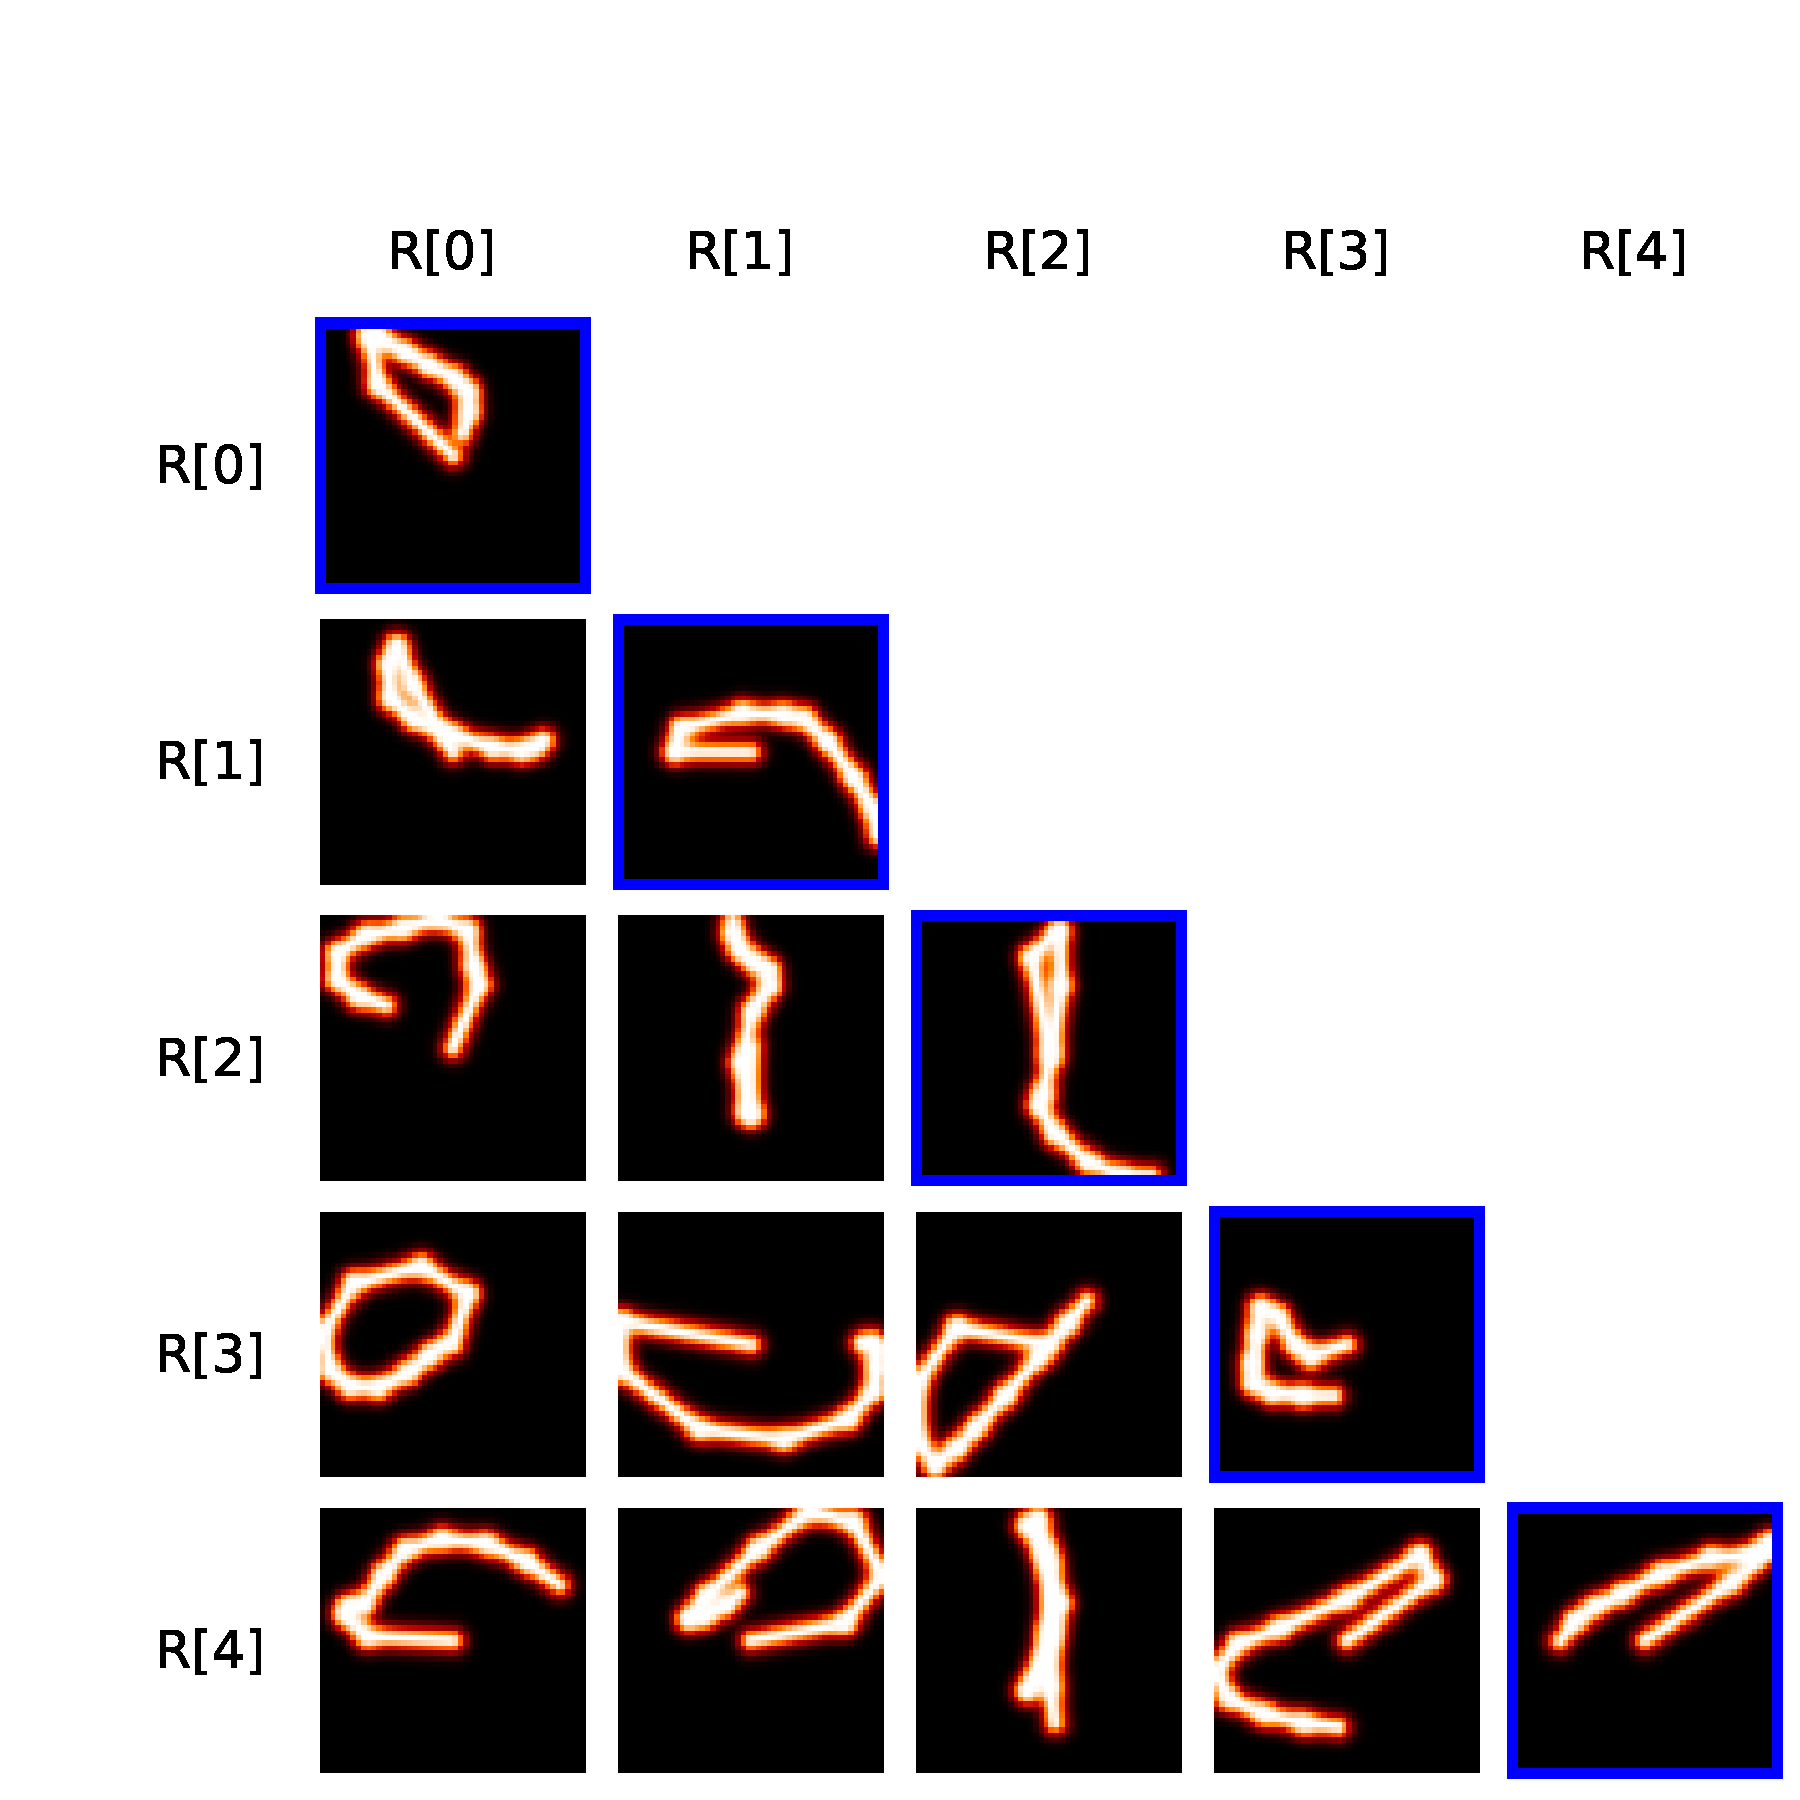
\includegraphics[width=0.4\textwidth]{curves/compo_m/compo0.pdf} & 
     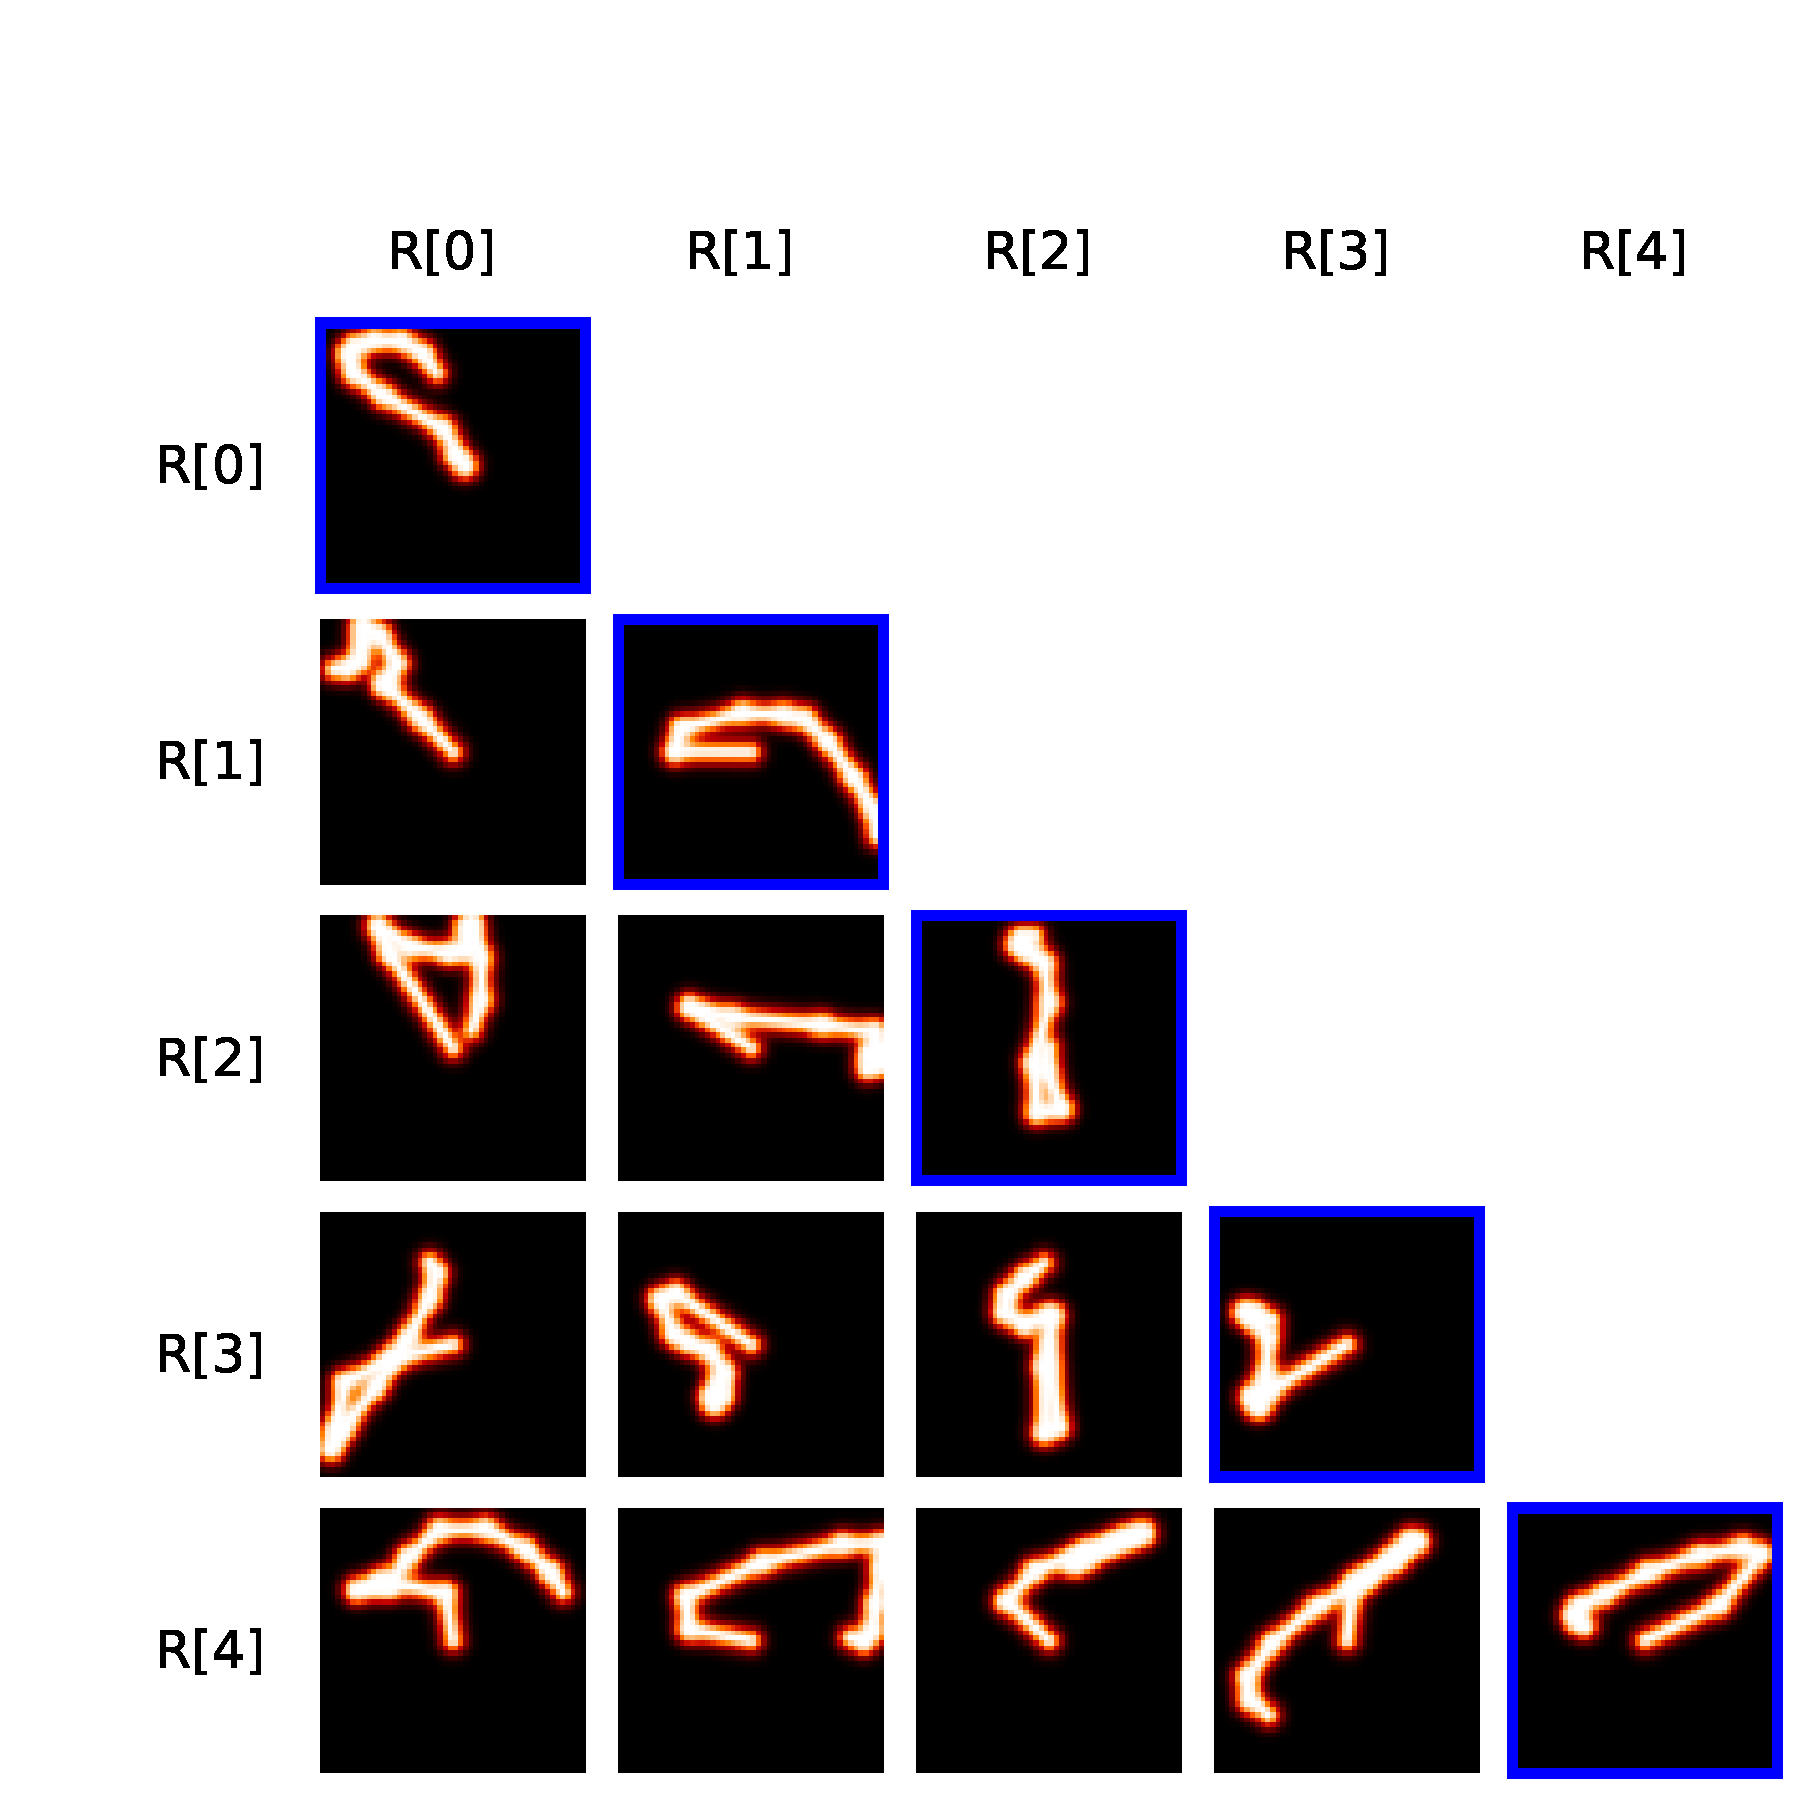
\includegraphics[width=0.4\textwidth]{curves/compo_m/compo1.pdf} \\
     \includegraphics[width=0.4\textwidth]{curves/compo_m/compo2.pdf}  &
     \includegraphics[width=0.4\textwidth]{curves/compo_m/compo3.pdf}  \\
     \includegraphics[width=0.4\textwidth]{curves/compo_m/compo4.pdf} &  
     \includegraphics[width=0.4\textwidth]{curves/compo_m/compo5.pdf} \\
    
 \end{tabular}

\caption{Instances of descriptive utterances for referents from $R_1$ (blue frames) and $R_2$.}
\end{figure}

\newpage
\subsection{T-SNEs of embeddings (Visual - Unshared Perspectives)}
\label{sup:tsnes}

\subsubsection{$R_2$ referents \& descriptive utterances}

\begin{figure}[h!]
\centering 

 \begin{tabular}{cc}

     \includegraphics[width=0.5\textwidth]{curves/tsnes/descriptive/9-TSNE-R2-R01.pdf} & 
     \includegraphics[width=0.5\textwidth]{curves/tsnes/descriptive/9-TSNE-R2-R02.pdf} \\
     \includegraphics[width=0.5\textwidth]{curves/tsnes/descriptive/9-TSNE-R2-R03.pdf}  &
     \includegraphics[width=0.5\textwidth]{curves/tsnes/descriptive/9-TSNE-R2-R04.pdf}  \\
     \includegraphics[width=0.5\textwidth]{curves/tsnes/descriptive/9-TSNE-R2-R12.pdf} &  
     \includegraphics[width=0.5\textwidth]{curves/tsnes/descriptive/9-TSNE-R2-R13.pdf}    \\
     \includegraphics[width=0.5\textwidth]{curves/tsnes/descriptive/9-TSNE-R2-R14.pdf} & 
     \includegraphics[width=0.5\textwidth]{curves/tsnes/descriptive/9-TSNE-R2-R23.pdf} \\
     \includegraphics[width=0.5\textwidth]{curves/tsnes/descriptive/9-TSNE-R2-R24.pdf}  &
     \includegraphics[width=0.5\textwidth]{curves/tsnes/descriptive/9-TSNE-R2-R34.pdf}
    
 \end{tabular}

\caption{\textbf{T-sne of referent and descriptive utterance embeddings.} Embeddings are computed for 100 perspectives of referents from $R_2$. Training conditions are unshared visual referents.}
\end{figure}

\newpage

\subsubsection{$R_2$ referents \& discriminative utterances}

\begin{figure}[h!]
 \begin{tabular}{cc}

     \includegraphics[width=0.5\textwidth]{curves/tsnes/discriminativ/9-TSNE-R2-R01.pdf} & 
     \includegraphics[width=0.5\textwidth]{curves/tsnes/discriminativ/9-TSNE-R2-R02.pdf} \\
     \includegraphics[width=0.5\textwidth]{curves/tsnes/discriminativ/9-TSNE-R2-R03.pdf}  &
     \includegraphics[width=0.5\textwidth]{curves/tsnes/discriminativ/9-TSNE-R2-R04.pdf}  \\
     \includegraphics[width=0.5\textwidth]{curves/tsnes/discriminativ/9-TSNE-R2-R12.pdf} &  
     \includegraphics[width=0.5\textwidth]{curves/tsnes/discriminativ/9-TSNE-R2-R13.pdf}    \\
     \includegraphics[width=0.5\textwidth]{curves/tsnes/discriminativ/9-TSNE-R2-R14.pdf} & 
     \includegraphics[width=0.5\textwidth]{curves/tsnes/discriminativ/9-TSNE-R2-R23.pdf} \\
     \includegraphics[width=0.5\textwidth]{curves/tsnes/discriminativ/9-TSNE-R2-R24.pdf}  &
     \includegraphics[width=0.5\textwidth]{curves/tsnes/discriminativ/9-TSNE-R2-R34.pdf}
    
 \end{tabular}
\caption{\textbf{T-sne of referent and discriminative utterance embeddings.}  Embeddings are computed for 100 perspectives of referents from $R_2$. Training conditions are unshared visual referents.}
\end{figure}

\end{document}